\pdfoutput=1
\documentclass[11pt]{article}

\usepackage[utf8]{inputenc}
\usepackage[T1]{fontenc}
\usepackage{lmodern}
\usepackage[margin=2.5cm]{geometry}
\usepackage{amsmath,amssymb}
\usepackage{graphicx}
\usepackage{booktabs}
\usepackage{tabularx}
\usepackage{xltabular}
\usepackage{threeparttable}
\usepackage{array}
\usepackage[final]{microtype}
\emergencystretch=1.5em
\usepackage{siunitx}
\usepackage{xcolor}
\usepackage{fancyhdr}
\usepackage{float}
\usepackage{enumitem}
\usepackage[square,comma,authoryear]{natbib}
\usepackage{xurl}
\usepackage[hidelinks]{hyperref}

\sisetup{group-separator={\,},output-decimal-marker={.}}
\setlist{itemsep=2pt,topsep=4pt}
\graphicspath{{../figures/}}
% generated by model/make_numbers.py -- do not edit
\makeatletter
\newcommand{\val}[1]{\@ifundefined{val@#1}{\textbf{??#1??}\PackageWarning{numbers}{undefined value #1}}{\@nameuse{val@#1}}}
\@namedef{val@afrrpool-2023}{0.0}
\@namedef{val@afrrpool-2024}{13.5}
\@namedef{val@afrrpool-2025}{24.6}
\@namedef{val@afrrpool-2026}{20.0}
\@namedef{val@ann-1-2026}{45.1}
\@namedef{val@ann-1-2030}{37.7}
\@namedef{val@ann-1-2035}{34.0}
\@namedef{val@ann-1-2040}{32.5}
\@namedef{val@ann-1-2045}{31.4}
\@namedef{val@ann-1-2050}{30.3}
\@namedef{val@ann-2-2026}{64.7}
\@namedef{val@ann-2-2030}{52.8}
\@namedef{val@ann-2-2035}{46.4}
\@namedef{val@ann-2-2040}{43.8}
\@namedef{val@ann-2-2045}{41.9}
\@namedef{val@ann-2-2050}{40.2}
\@namedef{val@ann-4-2026}{103.9}
\@namedef{val@ann-4-2030}{82.9}
\@namedef{val@ann-4-2035}{71.0}
\@namedef{val@ann-4-2040}{66.4}
\@namedef{val@ann-4-2045}{63.0}
\@namedef{val@ann-4-2050}{59.9}
\@namedef{val@ann-8-2026}{182.2}
\@namedef{val@ann-8-2030}{143.1}
\@namedef{val@ann-8-2035}{120.2}
\@namedef{val@ann-8-2040}{111.6}
\@namedef{val@ann-8-2045}{105.2}
\@namedef{val@ann-8-2050}{99.4}
\@namedef{val@ann-inc-24-2026}{39.2}
\@namedef{val@aux-2025}{1.8}
\@namedef{val@aux-2050}{1.3}
\@namedef{val@aux-share-2050}{37}
\@namedef{val@be-1-2026}{137}
\@namedef{val@be-1-2030}{115}
\@namedef{val@be-1-2035}{104}
\@namedef{val@be-1-2040}{99}
\@namedef{val@be-1-2045}{95}
\@namedef{val@be-1-2050}{92}
\@namedef{val@be-2-2026}{99}
\@namedef{val@be-2-2030}{80}
\@namedef{val@be-2-2035}{71}
\@namedef{val@be-2-2040}{67}
\@namedef{val@be-2-2045}{64}
\@namedef{val@be-2-2050}{61}
\@namedef{val@be-4-2026}{79}
\@namedef{val@be-4-2030}{63}
\@namedef{val@be-4-2035}{54}
\@namedef{val@be-4-2040}{51}
\@namedef{val@be-4-2045}{48}
\@namedef{val@be-4-2050}{46}
\@namedef{val@be-8-2026}{69}
\@namedef{val@be-8-2030}{54}
\@namedef{val@be-8-2035}{46}
\@namedef{val@be-8-2040}{42}
\@namedef{val@be-8-2045}{40}
\@namedef{val@be-8-2050}{38}
\@namedef{val@cE}{128.5}
\@namedef{val@cP}{75.0}
\@namedef{val@cap-first}{1\,269}
\@namedef{val@cap-first-month}{2026-03}
\@namedef{val@capex-1-2026}{405}
\@namedef{val@capex-1-2030}{340}
\@namedef{val@capex-1-2035}{309}
\@namedef{val@capex-1-2040}{295}
\@namedef{val@capex-1-2045}{286}
\@namedef{val@capex-1-2050}{277}
\@namedef{val@capex-2-2026}{285}
\@namedef{val@capex-2-2030}{233}
\@namedef{val@capex-2-2035}{205}
\@namedef{val@capex-2-2040}{194}
\@namedef{val@capex-2-2045}{187}
\@namedef{val@capex-2-2050}{179}
\@namedef{val@capex-4-2026}{225}
\@namedef{val@capex-4-2030}{179}
\@namedef{val@capex-4-2035}{154}
\@namedef{val@capex-4-2040}{144}
\@namedef{val@capex-4-2045}{137}
\@namedef{val@capex-4-2050}{131}
\@namedef{val@capex-4-high-2026}{274}
\@namedef{val@capex-4-high-2030}{237}
\@namedef{val@capex-4-high-2035}{217}
\@namedef{val@capex-4-high-2040}{209}
\@namedef{val@capex-4-high-2045}{204}
\@namedef{val@capex-4-high-2050}{200}
\@namedef{val@capex-4-low-2026}{193}
\@namedef{val@capex-4-low-2030}{140}
\@namedef{val@capex-4-low-2035}{111}
\@namedef{val@capex-4-low-2040}{99}
\@namedef{val@capex-4-low-2045}{93}
\@namedef{val@capex-4-low-2050}{88}
\@namedef{val@capex-8-2026}{195}
\@namedef{val@capex-8-2030}{153}
\@namedef{val@capex-8-2035}{128}
\@namedef{val@capex-8-2040}{119}
\@namedef{val@capex-8-2045}{112}
\@namedef{val@capex-8-2050}{106}
\@namedef{val@capture-central}{0.85}
\@namedef{val@charge-adder}{52}
\@namedef{val@comp-ce-2030}{96}
\@namedef{val@comp-ce-2035}{77}
\@namedef{val@comp-ce-2040}{72}
\@namedef{val@comp-ce-2050}{64}
\@namedef{val@comp-cells-2025}{36.0}
\@namedef{val@comp-cells-2030}{24}
\@namedef{val@comp-cells-2035}{19}
\@namedef{val@comp-cells-2040}{18}
\@namedef{val@comp-cells-2050}{18}
\@namedef{val@comp-cp-2030}{54}
\@namedef{val@comp-cp-2035}{46}
\@namedef{val@comp-cp-2040}{42}
\@namedef{val@comp-cp-2050}{37}
\@namedef{val@comp-dcbos-2025}{16.0}
\@namedef{val@comp-dcbos-2030}{11}
\@namedef{val@comp-dcbos-2035}{10}
\@namedef{val@comp-dcbos-2040}{9}
\@namedef{val@comp-dcbos-2050}{8}
\@namedef{val@comp-freight-2025}{7.0}
\@namedef{val@comp-premium-2025}{69.5}
\@namedef{val@comp-premium-2030}{54}
\@namedef{val@comp-premium-2035}{42}
\@namedef{val@comp-premium-2040}{38}
\@namedef{val@comp-premium-2050}{31}
\@namedef{val@cyc-2025}{17.7}
\@namedef{val@cyc-2025-high}{36.1}
\@namedef{val@cyc-2025-low}{8.1}
\@namedef{val@cyc-2026}{17.1}
\@namedef{val@cyc-2030}{13.1}
\@namedef{val@cyc-2035}{10.6}
\@namedef{val@cyc-2040}{9.9}
\@namedef{val@cyc-2045}{9.2}
\@namedef{val@cyc-2050}{8.7}
\@namedef{val@da-1-2023}{24.8}
\@namedef{val@da-1-2024}{27.9}
\@namedef{val@da-1-2025}{30.1}
\@namedef{val@da-1-2026}{33.3}
\@namedef{val@da-2-2023}{43.2}
\@namedef{val@da-2-2024}{50.2}
\@namedef{val@da-2-2025}{53.7}
\@namedef{val@da-2-2026}{53.5}
\@namedef{val@da-4-2023}{71.4}
\@namedef{val@da-4-2024}{82.2}
\@namedef{val@da-4-2025}{88.5}
\@namedef{val@da-4-2026}{83.9}
\@namedef{val@da-8-2023}{99.4}
\@namedef{val@da-8-2024}{111.4}
\@namedef{val@da-8-2025}{119.3}
\@namedef{val@da-8-2026}{109.9}
\@namedef{val@dam-1}{30.5}
\@namedef{val@dam-2}{52.5}
\@namedef{val@dam-4}{84.9}
\@namedef{val@dam-8}{113.5}
\@namedef{val@dam-inc-24}{32.4}
\@namedef{val@dam-inc-24-cap}{27.5}
\@namedef{val@daratio-1-2023}{55}
\@namedef{val@daratio-1-2024}{62}
\@namedef{val@daratio-1-2025}{67}
\@namedef{val@daratio-1-2026}{74}
\@namedef{val@daratio-2-2023}{67}
\@namedef{val@daratio-2-2024}{78}
\@namedef{val@daratio-2-2025}{83}
\@namedef{val@daratio-2-2026}{83}
\@namedef{val@daratio-4-2023}{69}
\@namedef{val@daratio-4-2024}{79}
\@namedef{val@daratio-4-2025}{85}
\@namedef{val@daratio-4-2026}{81}
\@namedef{val@daratio-8-2023}{55}
\@namedef{val@daratio-8-2024}{61}
\@namedef{val@daratio-8-2025}{65}
\@namedef{val@daratio-8-2026}{60}
\@namedef{val@daratio-max}{85}
\@namedef{val@daratio-min}{55}
\@namedef{val@doi}{10.5281/zenodo.24322467}
\@namedef{val@floor-2028}{3.6}
\@namedef{val@floor-2035}{3.6}
\@namedef{val@floor-2040}{2.1}
\@namedef{val@idxA-2025}{1.00}
\@namedef{val@idxA-2030}{0.78}
\@namedef{val@idxA-2035}{0.61}
\@namedef{val@idxA-2040}{0.55}
\@namedef{val@idxA-2050}{0.45}
\@namedef{val@idxB-2025}{1.00}
\@namedef{val@idxB-2030}{0.71}
\@namedef{val@idxB-2035}{0.50}
\@namedef{val@idxB-2040}{0.44}
\@namedef{val@idxB-2050}{0.34}
\@namedef{val@idxC-central-2026}{1.00}
\@namedef{val@idxC-central-2027}{0.97}
\@namedef{val@idxC-central-2030}{0.74}
\@namedef{val@idxC-central-2035}{0.60}
\@namedef{val@idxC-central-2040}{0.56}
\@namedef{val@idxC-central-2050}{0.49}
\@namedef{val@idxC-high-2030}{0.89}
\@namedef{val@idxC-high-2035}{0.80}
\@namedef{val@idxC-high-2040}{0.77}
\@namedef{val@idxC-high-2050}{0.72}
\@namedef{val@idxC-low-2030}{0.62}
\@namedef{val@idxC-low-2035}{0.44}
\@namedef{val@idxC-low-2040}{0.38}
\@namedef{val@idxC-low-2050}{0.33}
\@namedef{val@idxC-premhigh-2030}{0.80}
\@namedef{val@idxC-premhigh-2035}{0.71}
\@namedef{val@idxC-premhigh-2040}{0.67}
\@namedef{val@idxC-premhigh-2050}{0.62}
\@namedef{val@idxC-premlow-2030}{0.66}
\@namedef{val@idxC-premlow-2035}{0.48}
\@namedef{val@idxC-premlow-2040}{0.44}
\@namedef{val@idxC-premlow-2050}{0.39}
\@namedef{val@lcos-2-2026}{144}
\@namedef{val@lcos-2-2030}{117}
\@namedef{val@lcos-2-2035}{103}
\@namedef{val@lcos-2-2040}{97}
\@namedef{val@lcos-2-2045}{93}
\@namedef{val@lcos-2-2050}{89}
\@namedef{val@lcos-4-2026}{115}
\@namedef{val@lcos-4-2030}{92}
\@namedef{val@lcos-4-2035}{79}
\@namedef{val@lcos-4-2040}{74}
\@namedef{val@lcos-4-2045}{70}
\@namedef{val@lcos-4-2050}{67}
\@namedef{val@loo-M1-2027}{5}
\@namedef{val@loo-M1-2028}{1}
\@namedef{val@loo-M1-2030}{$-$2}
\@namedef{val@loo-M2-2030}{$-$5}
\@namedef{val@loo-M2-2035}{$-$9}
\@namedef{val@loo-M2-2040}{$-$6}
\@namedef{val@loo-M2-2045}{$-$7}
\@namedef{val@loo-M2-2050}{$-$2}
\@namedef{val@loo-M3-2027}{4}
\@namedef{val@loo-M3-2028}{0}
\@namedef{val@loo-M3-2030}{4}
\@namedef{val@loo-M3-2035}{11}
\@namedef{val@loo-M3-2040}{33}
\@namedef{val@loo-M3-2045}{19}
\@namedef{val@loo-M3-2050}{6}
\@namedef{val@loo-M4-2035}{1}
\@namedef{val@loo-M4-2040}{0}
\@namedef{val@loo-M4-2045}{0}
\@namedef{val@loo-M4-2050}{0}
\@namedef{val@loo-M5-2027}{$-$1}
\@namedef{val@loo-M5-2028}{$-$1}
\@namedef{val@loo-M5-2030}{3}
\@namedef{val@loo-M5-2035}{$-$7}
\@namedef{val@loo-M5-2040}{$-$8}
\@namedef{val@loo-M5-2045}{$-$8}
\@namedef{val@loo-M5-2050}{$-$6}
\@namedef{val@loo-max-late}{33}
\@namedef{val@m-M1-gw-p10-2027}{2.7}
\@namedef{val@m-M1-gw-p10-2028}{3.6}
\@namedef{val@m-M1-gw-p10-2030}{4.3}
\@namedef{val@m-M1-gw-p50-2027}{3.0}
\@namedef{val@m-M1-gw-p50-2028}{3.9}
\@namedef{val@m-M1-gw-p50-2030}{4.9}
\@namedef{val@m-M1-gw-p90-2027}{3.3}
\@namedef{val@m-M1-gw-p90-2028}{4.1}
\@namedef{val@m-M1-gw-p90-2030}{5.5}
\@namedef{val@m-M1-gwh-p10-2027}{5.7}
\@namedef{val@m-M1-gwh-p10-2028}{8.3}
\@namedef{val@m-M1-gwh-p10-2030}{10.2}
\@namedef{val@m-M1-gwh-p50-2027}{6.6}
\@namedef{val@m-M1-gwh-p50-2028}{9.1}
\@namedef{val@m-M1-gwh-p50-2030}{11.9}
\@namedef{val@m-M1-gwh-p90-2027}{7.5}
\@namedef{val@m-M1-gwh-p90-2028}{9.5}
\@namedef{val@m-M1-gwh-p90-2030}{13.8}
\@namedef{val@m-M2-gw-p10-2030}{4.6}
\@namedef{val@m-M2-gw-p10-2035}{4.9}
\@namedef{val@m-M2-gw-p10-2040}{4.9}
\@namedef{val@m-M2-gw-p10-2045}{4.9}
\@namedef{val@m-M2-gw-p10-2050}{4.9}
\@namedef{val@m-M2-gw-p50-2030}{5.8}
\@namedef{val@m-M2-gw-p50-2035}{9.9}
\@namedef{val@m-M2-gw-p50-2040}{10.9}
\@namedef{val@m-M2-gw-p50-2045}{11.1}
\@namedef{val@m-M2-gw-p50-2050}{11.1}
\@namedef{val@m-M2-gw-p90-2030}{6.8}
\@namedef{val@m-M2-gw-p90-2035}{16.0}
\@namedef{val@m-M2-gw-p90-2040}{22.5}
\@namedef{val@m-M2-gw-p90-2045}{24.5}
\@namedef{val@m-M2-gw-p90-2050}{25.0}
\@namedef{val@m-M2-gwh-p10-2030}{11.1}
\@namedef{val@m-M2-gwh-p10-2035}{12.1}
\@namedef{val@m-M2-gwh-p10-2040}{12.2}
\@namedef{val@m-M2-gwh-p10-2045}{12.2}
\@namedef{val@m-M2-gwh-p10-2050}{12.2}
\@namedef{val@m-M2-gwh-p50-2030}{14.7}
\@namedef{val@m-M2-gwh-p50-2035}{27.7}
\@namedef{val@m-M2-gwh-p50-2040}{31.7}
\@namedef{val@m-M2-gwh-p50-2045}{32.4}
\@namedef{val@m-M2-gwh-p50-2050}{32.5}
\@namedef{val@m-M2-gwh-p90-2030}{17.8}
\@namedef{val@m-M2-gwh-p90-2035}{48.3}
\@namedef{val@m-M2-gwh-p90-2040}{71.1}
\@namedef{val@m-M2-gwh-p90-2045}{79.2}
\@namedef{val@m-M2-gwh-p90-2050}{81.4}
\@namedef{val@m-M3-gw-p10-2027}{3.2}
\@namedef{val@m-M3-gw-p10-2028}{3.9}
\@namedef{val@m-M3-gw-p10-2030}{4.0}
\@namedef{val@m-M3-gw-p10-2035}{4.2}
\@namedef{val@m-M3-gw-p10-2040}{4.0}
\@namedef{val@m-M3-gw-p10-2045}{4.7}
\@namedef{val@m-M3-gw-p10-2050}{5.4}
\@namedef{val@m-M3-gw-p50-2027}{3.2}
\@namedef{val@m-M3-gw-p50-2028}{4.0}
\@namedef{val@m-M3-gw-p50-2030}{4.2}
\@namedef{val@m-M3-gw-p50-2035}{5.1}
\@namedef{val@m-M3-gw-p50-2040}{6.2}
\@namedef{val@m-M3-gw-p50-2045}{7.6}
\@namedef{val@m-M3-gw-p50-2050}{9.1}
\@namedef{val@m-M3-gw-p90-2027}{3.4}
\@namedef{val@m-M3-gw-p90-2028}{4.1}
\@namedef{val@m-M3-gw-p90-2030}{5.0}
\@namedef{val@m-M3-gw-p90-2035}{8.7}
\@namedef{val@m-M3-gw-p90-2040}{11.9}
\@namedef{val@m-M3-gw-p90-2045}{15.3}
\@namedef{val@m-M3-gw-p90-2050}{19.2}
\@namedef{val@m-M3-gwh-p10-2027}{7.0}
\@namedef{val@m-M3-gwh-p10-2028}{9.1}
\@namedef{val@m-M3-gwh-p10-2030}{9.1}
\@namedef{val@m-M3-gwh-p10-2035}{9.4}
\@namedef{val@m-M3-gwh-p10-2040}{8.8}
\@namedef{val@m-M3-gwh-p10-2045}{11.4}
\@namedef{val@m-M3-gwh-p10-2050}{13.5}
\@namedef{val@m-M3-gwh-p50-2027}{7.1}
\@namedef{val@m-M3-gwh-p50-2028}{9.1}
\@namedef{val@m-M3-gwh-p50-2030}{9.3}
\@namedef{val@m-M3-gwh-p50-2035}{11.6}
\@namedef{val@m-M3-gwh-p50-2040}{17.1}
\@namedef{val@m-M3-gwh-p50-2045}{25.5}
\@namedef{val@m-M3-gwh-p50-2050}{31.6}
\@namedef{val@m-M3-gwh-p90-2027}{7.3}
\@namedef{val@m-M3-gwh-p90-2028}{9.4}
\@namedef{val@m-M3-gwh-p90-2030}{11.2}
\@namedef{val@m-M3-gwh-p90-2035}{24.7}
\@namedef{val@m-M3-gwh-p90-2040}{39.0}
\@namedef{val@m-M3-gwh-p90-2045}{57.1}
\@namedef{val@m-M3-gwh-p90-2050}{75.3}
\@namedef{val@m-M4-gw-p10-2035}{3.6}
\@namedef{val@m-M4-gw-p10-2040}{3.3}
\@namedef{val@m-M4-gw-p10-2045}{3.9}
\@namedef{val@m-M4-gw-p10-2050}{4.6}
\@namedef{val@m-M4-gw-p50-2035}{4.9}
\@namedef{val@m-M4-gw-p50-2040}{6.1}
\@namedef{val@m-M4-gw-p50-2045}{7.0}
\@namedef{val@m-M4-gw-p50-2050}{8.1}
\@namedef{val@m-M4-gw-p90-2035}{10.5}
\@namedef{val@m-M4-gw-p90-2040}{12.7}
\@namedef{val@m-M4-gw-p90-2045}{14.5}
\@namedef{val@m-M4-gw-p90-2050}{16.3}
\@namedef{val@m-M4-gwh-p10-2035}{8.3}
\@namedef{val@m-M4-gwh-p10-2040}{7.4}
\@namedef{val@m-M4-gwh-p10-2045}{9.2}
\@namedef{val@m-M4-gwh-p10-2050}{12.1}
\@namedef{val@m-M4-gwh-p50-2035}{12.0}
\@namedef{val@m-M4-gwh-p50-2040}{16.1}
\@namedef{val@m-M4-gwh-p50-2045}{20.5}
\@namedef{val@m-M4-gwh-p50-2050}{26.1}
\@namedef{val@m-M4-gwh-p90-2035}{30.1}
\@namedef{val@m-M4-gwh-p90-2040}{39.1}
\@namedef{val@m-M4-gwh-p90-2045}{46.6}
\@namedef{val@m-M4-gwh-p90-2050}{54.4}
\@namedef{val@m-M5-gw-p10-2027}{3.4}
\@namedef{val@m-M5-gw-p10-2028}{3.7}
\@namedef{val@m-M5-gw-p10-2030}{3.8}
\@namedef{val@m-M5-gw-p10-2035}{5.7}
\@namedef{val@m-M5-gw-p10-2040}{6.7}
\@namedef{val@m-M5-gw-p10-2045}{6.7}
\@namedef{val@m-M5-gw-p10-2050}{6.7}
\@namedef{val@m-M5-gw-p50-2027}{3.8}
\@namedef{val@m-M5-gw-p50-2028}{4.2}
\@namedef{val@m-M5-gw-p50-2030}{4.5}
\@namedef{val@m-M5-gw-p50-2035}{7.5}
\@namedef{val@m-M5-gw-p50-2040}{10.9}
\@namedef{val@m-M5-gw-p50-2045}{10.9}
\@namedef{val@m-M5-gw-p50-2050}{10.9}
\@namedef{val@m-M5-gw-p90-2027}{4.2}
\@namedef{val@m-M5-gw-p90-2028}{4.8}
\@namedef{val@m-M5-gw-p90-2030}{5.2}
\@namedef{val@m-M5-gw-p90-2035}{9.4}
\@namedef{val@m-M5-gw-p90-2040}{32.3}
\@namedef{val@m-M5-gw-p90-2045}{32.3}
\@namedef{val@m-M5-gw-p90-2050}{32.3}
\@namedef{val@m-M5-gwh-p10-2027}{7.7}
\@namedef{val@m-M5-gwh-p10-2028}{8.5}
\@namedef{val@m-M5-gwh-p10-2030}{8.8}
\@namedef{val@m-M5-gwh-p10-2035}{19.5}
\@namedef{val@m-M5-gwh-p10-2040}{24.9}
\@namedef{val@m-M5-gwh-p10-2045}{24.9}
\@namedef{val@m-M5-gwh-p10-2050}{24.9}
\@namedef{val@m-M5-gwh-p50-2027}{8.8}
\@namedef{val@m-M5-gwh-p50-2028}{10.0}
\@namedef{val@m-M5-gwh-p50-2030}{12.3}
\@namedef{val@m-M5-gwh-p50-2035}{29.3}
\@namedef{val@m-M5-gwh-p50-2040}{50.5}
\@namedef{val@m-M5-gwh-p50-2045}{50.5}
\@namedef{val@m-M5-gwh-p50-2050}{50.5}
\@namedef{val@m-M5-gwh-p90-2027}{9.9}
\@namedef{val@m-M5-gwh-p90-2028}{11.4}
\@namedef{val@m-M5-gwh-p90-2030}{16.9}
\@namedef{val@m-M5-gwh-p90-2035}{43.7}
\@namedef{val@m-M5-gwh-p90-2040}{193.5}
\@namedef{val@m-M5-gwh-p90-2045}{193.5}
\@namedef{val@m-M5-gwh-p90-2050}{193.5}
\@namedef{val@m2-dt-p10}{6}
\@namedef{val@m2-dt-p50}{11.2}
\@namedef{val@m2-dt-p90}{14}
\@namedef{val@m3-npar}{17}
\@namedef{val@m3c-first4h}{2035}
\@namedef{val@m3c-gw-2030}{4.0}
\@namedef{val@m3c-gw-2035}{4.6}
\@namedef{val@m3c-gw-2040}{5.6}
\@namedef{val@m3c-gw-2050}{7.9}
\@namedef{val@m3c-gwh-2030}{9.2}
\@namedef{val@m3c-gwh-2035}{10.8}
\@namedef{val@m3c-gwh-2040}{16.9}
\@namedef{val@m3c-gwh-2050}{29.2}
\@namedef{val@m3c-nstar-2026}{2.38}
\@namedef{val@m3c-nstar-2030}{3.4}
\@namedef{val@m3c-nstar-2035}{4.3}
\@namedef{val@m3c-nstar-2040}{5.1}
\@namedef{val@m3c-nstar-2050}{7.1}
\@namedef{val@m3d1-2030}{0}
\@namedef{val@m3d1-2035}{0}
\@namedef{val@m3d1-2040}{0}
\@namedef{val@m3d1-2045}{0}
\@namedef{val@m3d1-2050}{0}
\@namedef{val@m3d2-2030}{94}
\@namedef{val@m3d2-2035}{33}
\@namedef{val@m3d2-2040}{17}
\@namedef{val@m3d2-2045}{10}
\@namedef{val@m3d2-2050}{6}
\@namedef{val@m3d4-2030}{6}
\@namedef{val@m3d4-2035}{67}
\@namedef{val@m3d4-2040}{82}
\@namedef{val@m3d4-2045}{88}
\@namedef{val@m3d4-2050}{90}
\@namedef{val@m3d8-2030}{0}
\@namedef{val@m3d8-2035}{0}
\@namedef{val@m3d8-2040}{0}
\@namedef{val@m3d8-2045}{2}
\@namedef{val@m3d8-2050}{5}
\@namedef{val@mfrrpool-2023}{44.5}
\@namedef{val@mfrrpool-2024}{56.4}
\@namedef{val@mfrrpool-2025}{128.7}
\@namedef{val@mfrrpool-2026}{68.4}
\@namedef{val@mhr-2025}{0.71}
\@namedef{val@mhr-2035}{0.50}
\@namedef{val@mhr-2050}{0.42}
\@namedef{val@min-load-now}{24}
\@namedef{val@ndraws}{4\,000}
\@namedef{val@old-m-M3-gw-p50-2035}{4.7}
\@namedef{val@old-m3c-gw-2035}{4.3}
\@namedef{val@old-st-gw-base-2035}{7.2}
\@namedef{val@old-st-gw-base-2050}{10.5}
\@namedef{val@old-st-gw-low-2050}{4.6}
\@namedef{val@params-sha}{b44dfaef823bca0d}
\@namedef{val@pc-china}{0.12}
\@namedef{val@pc-fi-2050}{1.82}
\@namedef{val@pc-fi-2050-high}{3.89}
\@namedef{val@pc-fi-2050-low}{0.85}
\@namedef{val@pc-fi-2050-m3}{1.63}
\@namedef{val@pc-finland}{0.37}
\@namedef{val@pc-italy}{0.13}
\@namedef{val@pc-lithuania}{0.41}
\@namedef{val@pc-sweden}{0.09}
\@namedef{val@pc-united}{0.15}
\@namedef{val@pc-world}{0.06}
\@namedef{val@pc2050-denmark-x}{1.13}
\@namedef{val@pc2050-world-bnef}{0.40}
\@namedef{val@pc2050-world-x}{0.42}
\@namedef{val@poolsens0-base-2035}{7.0}
\@namedef{val@poolsens0-base-2050}{10.2}
\@namedef{val@poolsens0-high-2050}{21.8}
\@namedef{val@poolsens0-m4-p50-2050}{8.1}
\@namedef{val@poolsens1-base-2035}{7.0}
\@namedef{val@poolsens1-base-2050}{11.4}
\@namedef{val@poolsens1-high-2050}{21.8}
\@namedef{val@poolsens1-m4-p50-2050}{14.2}
\@namedef{val@poolsens2-base-2035}{7.0}
\@namedef{val@poolsens2-base-2050}{10.8}
\@namedef{val@poolsens2-high-2050}{21.8}
\@namedef{val@poolsens2-m4-p50-2050}{12.9}
\@namedef{val@poolsens3-base-2035}{7.0}
\@namedef{val@poolsens3-base-2050}{10.5}
\@namedef{val@poolsens3-high-2050}{27.3}
\@namedef{val@poolsens3-m4-p50-2050}{8.1}
\@namedef{val@prem-share-2025}{54}
\@namedef{val@res-hours-2026}{318}
\@namedef{val@respool-2023}{123.8}
\@namedef{val@respool-2024}{110.0}
\@namedef{val@respool-2025}{83.8}
\@namedef{val@respool-2026}{36.3}
\@namedef{val@seed}{20261116}
\@namedef{val@seed-base-max}{2.7}
\@namedef{val@seed-high-max}{5.7}
\@namedef{val@sf-1-2026-full}{7.4}
\@namedef{val@sf-1-2026-half}{3.7}
\@namedef{val@sf-1-2028-full}{9.0}
\@namedef{val@sf-1-2028-half}{4.5}
\@namedef{val@sf-1-2030-full}{13.2}
\@namedef{val@sf-1-2030-half}{6.6}
\@namedef{val@sf-1-2035-full}{21.7}
\@namedef{val@sf-1-2035-half}{10.8}
\@namedef{val@sf-1-2040-full}{29.8}
\@namedef{val@sf-1-2040-half}{14.9}
\@namedef{val@sf-2-2026-full}{6.5}
\@namedef{val@sf-2-2026-half}{3.2}
\@namedef{val@sf-2-2028-full}{8.7}
\@namedef{val@sf-2-2028-half}{4.4}
\@namedef{val@sf-2-2030-full}{17.1}
\@namedef{val@sf-2-2030-half}{8.5}
\@namedef{val@sf-2-2035-full}{143.8}
\@namedef{val@sf-2-2035-half}{71.9}
\@namedef{val@sf-2-2040-full}{inf}
\@namedef{val@sf-2-2040-half}{inf}
\@namedef{val@sf-4-2026-full}{3.8}
\@namedef{val@sf-4-2026-half}{1.9}
\@namedef{val@sf-4-2028-full}{5.3}
\@namedef{val@sf-4-2028-half}{2.6}
\@namedef{val@sf-4-2030-full}{10.7}
\@namedef{val@sf-4-2030-half}{5.4}
\@namedef{val@sf-4-2035-full}{inf}
\@namedef{val@sf-4-2035-half}{inf}
\@namedef{val@sf-4-2040-full}{inf}
\@namedef{val@sf-4-2040-half}{inf}
\@namedef{val@sf-8-2026-full}{1.4}
\@namedef{val@sf-8-2026-half}{0.7}
\@namedef{val@sf-8-2028-full}{1.7}
\@namedef{val@sf-8-2028-half}{0.9}
\@namedef{val@sf-8-2030-full}{2.5}
\@namedef{val@sf-8-2030-half}{1.3}
\@namedef{val@sf-8-2035-full}{4.7}
\@namedef{val@sf-8-2035-half}{2.3}
\@namedef{val@sf-8-2040-full}{6.9}
\@namedef{val@sf-8-2040-half}{3.4}
\@namedef{val@sha-cost}{e48566491506b6b5}
\@namedef{val@sha-ensemble}{9832a597d4f4f0bb}
\@namedef{val@sha-fequilibrium}{dc465fc4d812e046}
\@namedef{val@sha-fmethods}{d5a0dddc317173b2}
\@namedef{val@sob-build_limit-2035-gw-S1}{$-$0.01}
\@namedef{val@sob-build_limit-2035-gw-ST}{0.02}
\@namedef{val@sob-build_limit-2035-gwh-S1}{$-$0.01}
\@namedef{val@sob-build_limit-2035-gwh-ST}{0.03}
\@namedef{val@sob-build_limit-2050-gw-S1}{0.01}
\@namedef{val@sob-build_limit-2050-gw-ST}{0.07}
\@namedef{val@sob-build_limit-2050-gwh-S1}{0.01}
\@namedef{val@sob-build_limit-2050-gwh-ST}{0.06}
\@namedef{val@sob-capture-2035-gw-S1}{0.01}
\@namedef{val@sob-capture-2035-gw-ST}{0.02}
\@namedef{val@sob-capture-2035-gwh-S1}{0.01}
\@namedef{val@sob-capture-2035-gwh-ST}{0.02}
\@namedef{val@sob-capture-2050-gw-S1}{0.01}
\@namedef{val@sob-capture-2050-gw-ST}{0.01}
\@namedef{val@sob-capture-2050-gwh-S1}{0.01}
\@namedef{val@sob-capture-2050-gwh-ST}{0.01}
\@namedef{val@sob-cons_2035-2035-gw-S1}{0.04}
\@namedef{val@sob-cons_2035-2035-gw-ST}{0.07}
\@namedef{val@sob-cons_2035-2035-gwh-S1}{0.04}
\@namedef{val@sob-cons_2035-2035-gwh-ST}{0.09}
\@namedef{val@sob-cons_2035-2050-gw-S1}{0.00}
\@namedef{val@sob-cons_2035-2050-gw-ST}{0.00}
\@namedef{val@sob-cons_2035-2050-gwh-S1}{0.00}
\@namedef{val@sob-cons_2035-2050-gwh-ST}{0.00}
\@namedef{val@sob-cons_2050-2035-gw-S1}{0.00}
\@namedef{val@sob-cons_2050-2035-gw-ST}{0.00}
\@namedef{val@sob-cons_2050-2035-gwh-S1}{0.00}
\@namedef{val@sob-cons_2050-2035-gwh-ST}{0.00}
\@namedef{val@sob-cons_2050-2050-gw-S1}{0.01}
\@namedef{val@sob-cons_2050-2050-gw-ST}{0.04}
\@namedef{val@sob-cons_2050-2050-gwh-S1}{0.02}
\@namedef{val@sob-cons_2050-2050-gwh-ST}{0.05}
\@namedef{val@sob-cost_u-2035-gw-S1}{0.02}
\@namedef{val@sob-cost_u-2035-gw-ST}{0.03}
\@namedef{val@sob-cost_u-2035-gwh-S1}{0.02}
\@namedef{val@sob-cost_u-2035-gwh-ST}{0.04}
\@namedef{val@sob-cost_u-2050-gw-S1}{0.01}
\@namedef{val@sob-cost_u-2050-gw-ST}{0.02}
\@namedef{val@sob-cost_u-2050-gwh-S1}{0.01}
\@namedef{val@sob-cost_u-2050-gwh-ST}{0.03}
\@namedef{val@sob-duration_tilt-2035-gw-S1}{0.01}
\@namedef{val@sob-duration_tilt-2035-gw-ST}{0.01}
\@namedef{val@sob-duration_tilt-2035-gwh-S1}{0.02}
\@namedef{val@sob-duration_tilt-2035-gwh-ST}{0.03}
\@namedef{val@sob-duration_tilt-2050-gw-S1}{0.01}
\@namedef{val@sob-duration_tilt-2050-gw-ST}{0.01}
\@namedef{val@sob-duration_tilt-2050-gwh-S1}{0.04}
\@namedef{val@sob-duration_tilt-2050-gwh-ST}{0.09}
\@namedef{val@sob-eps_flex-2035-gw-S1}{0.13}
\@namedef{val@sob-eps_flex-2035-gw-ST}{0.20}
\@namedef{val@sob-eps_flex-2035-gwh-S1}{0.15}
\@namedef{val@sob-eps_flex-2035-gwh-ST}{0.26}
\@namedef{val@sob-eps_flex-2050-gw-S1}{0.22}
\@namedef{val@sob-eps_flex-2050-gw-ST}{0.28}
\@namedef{val@sob-eps_flex-2050-gwh-S1}{0.26}
\@namedef{val@sob-eps_flex-2050-gwh-ST}{0.35}
\@namedef{val@sob-eps_own-2035-gw-S1}{0.25}
\@namedef{val@sob-eps_own-2035-gw-ST}{0.45}
\@namedef{val@sob-eps_own-2035-gwh-S1}{0.27}
\@namedef{val@sob-eps_own-2035-gwh-ST}{0.48}
\@namedef{val@sob-eps_own-2050-gw-S1}{0.33}
\@namedef{val@sob-eps_own-2050-gw-ST}{0.48}
\@namedef{val@sob-eps_own-2050-gwh-S1}{0.29}
\@namedef{val@sob-eps_own-2050-gwh-ST}{0.43}
\@namedef{val@sob-eps_pool-2035-gw-S1}{0.00}
\@namedef{val@sob-eps_pool-2035-gw-ST}{0.00}
\@namedef{val@sob-eps_pool-2035-gwh-S1}{0.00}
\@namedef{val@sob-eps_pool-2035-gwh-ST}{0.00}
\@namedef{val@sob-eps_pool-2050-gw-S1}{0.00}
\@namedef{val@sob-eps_pool-2050-gw-ST}{0.00}
\@namedef{val@sob-eps_pool-2050-gwh-S1}{$-$0.00}
\@namedef{val@sob-eps_pool-2050-gwh-ST}{0.00}
\@namedef{val@sob-eps_pool_sat-2035-gw-S1}{0.00}
\@namedef{val@sob-eps_pool_sat-2035-gw-ST}{0.00}
\@namedef{val@sob-eps_pool_sat-2035-gwh-S1}{0.00}
\@namedef{val@sob-eps_pool_sat-2035-gwh-ST}{0.00}
\@namedef{val@sob-eps_pool_sat-2050-gw-S1}{0.00}
\@namedef{val@sob-eps_pool_sat-2050-gw-ST}{0.00}
\@namedef{val@sob-eps_pool_sat-2050-gwh-S1}{0.00}
\@namedef{val@sob-eps_pool_sat-2050-gwh-ST}{0.00}
\@namedef{val@sob-finance_u-2035-gw-S1}{0.14}
\@namedef{val@sob-finance_u-2035-gw-ST}{0.24}
\@namedef{val@sob-finance_u-2035-gwh-S1}{0.11}
\@namedef{val@sob-finance_u-2035-gwh-ST}{0.20}
\@namedef{val@sob-finance_u-2050-gw-S1}{0.08}
\@namedef{val@sob-finance_u-2050-gw-ST}{0.11}
\@namedef{val@sob-finance_u-2050-gwh-S1}{0.06}
\@namedef{val@sob-finance_u-2050-gwh-ST}{0.09}
\@namedef{val@sob-grid_forming-2035-gw-S1}{0.00}
\@namedef{val@sob-grid_forming-2035-gw-ST}{0.01}
\@namedef{val@sob-grid_forming-2035-gwh-S1}{$-$0.00}
\@namedef{val@sob-grid_forming-2035-gwh-ST}{0.00}
\@namedef{val@sob-grid_forming-2050-gw-S1}{0.00}
\@namedef{val@sob-grid_forming-2050-gw-ST}{0.00}
\@namedef{val@sob-grid_forming-2050-gwh-S1}{0.00}
\@namedef{val@sob-grid_forming-2050-gwh-ST}{0.00}
\@namedef{val@sob-phes-2035-gw-S1}{0.02}
\@namedef{val@sob-phes-2035-gw-ST}{0.01}
\@namedef{val@sob-phes-2035-gwh-S1}{0.01}
\@namedef{val@sob-phes-2035-gwh-ST}{0.01}
\@namedef{val@sob-phes-2050-gw-S1}{0.01}
\@namedef{val@sob-phes-2050-gw-ST}{0.00}
\@namedef{val@sob-phes-2050-gwh-S1}{0.00}
\@namedef{val@sob-phes-2050-gwh-ST}{0.00}
\@namedef{val@sob-pool_share-2035-gw-S1}{0.01}
\@namedef{val@sob-pool_share-2035-gw-ST}{0.01}
\@namedef{val@sob-pool_share-2035-gwh-S1}{0.00}
\@namedef{val@sob-pool_share-2035-gwh-ST}{0.00}
\@namedef{val@sob-pool_share-2050-gw-S1}{0.00}
\@namedef{val@sob-pool_share-2050-gw-ST}{0.00}
\@namedef{val@sob-pool_share-2050-gwh-S1}{$-$0.00}
\@namedef{val@sob-pool_share-2050-gwh-ST}{0.00}
\@namedef{val@sob-premium_u-2035-gw-S1}{0.02}
\@namedef{val@sob-premium_u-2035-gw-ST}{0.05}
\@namedef{val@sob-premium_u-2035-gwh-S1}{0.02}
\@namedef{val@sob-premium_u-2035-gwh-ST}{0.06}
\@namedef{val@sob-premium_u-2050-gw-S1}{0.02}
\@namedef{val@sob-premium_u-2050-gw-ST}{0.03}
\@namedef{val@sob-premium_u-2050-gwh-S1}{0.03}
\@namedef{val@sob-premium_u-2050-gwh-ST}{0.05}
\@namedef{val@sob-project_u-2035-gw-S1}{0.08}
\@namedef{val@sob-project_u-2035-gw-ST}{0.15}
\@namedef{val@sob-project_u-2035-gwh-S1}{0.05}
\@namedef{val@sob-project_u-2035-gwh-ST}{0.10}
\@namedef{val@sob-project_u-2050-gw-S1}{0.06}
\@namedef{val@sob-project_u-2050-gw-ST}{0.09}
\@namedef{val@sob-project_u-2050-gwh-S1}{0.03}
\@namedef{val@sob-project_u-2050-gwh-ST}{0.06}
\@namedef{val@sob-vre_mult-2035-gw-S1}{0.01}
\@namedef{val@sob-vre_mult-2035-gw-ST}{0.02}
\@namedef{val@sob-vre_mult-2035-gwh-S1}{0.01}
\@namedef{val@sob-vre_mult-2035-gwh-ST}{0.02}
\@namedef{val@sob-vre_mult-2050-gw-S1}{0.03}
\@namedef{val@sob-vre_mult-2050-gw-ST}{0.05}
\@namedef{val@sob-vre_mult-2050-gwh-S1}{0.04}
\@namedef{val@sob-vre_mult-2050-gwh-ST}{0.07}
\@namedef{val@sobol-evals}{155\,648}
\@namedef{val@sobol-se-max}{0.035}
\@namedef{val@sobolbase}{8\,192}
\@namedef{val@st-dur-base-2027}{2.2}
\@namedef{val@st-dur-base-2028}{2.3}
\@namedef{val@st-dur-base-2030}{2.5}
\@namedef{val@st-dur-base-2035}{2.7}
\@namedef{val@st-dur-base-2040}{2.9}
\@namedef{val@st-dur-base-2045}{3.2}
\@namedef{val@st-dur-base-2050}{3.3}
\@namedef{val@st-dur-high-2027}{2.3}
\@namedef{val@st-dur-high-2028}{2.4}
\@namedef{val@st-dur-high-2030}{2.8}
\@namedef{val@st-dur-high-2035}{4.1}
\@namedef{val@st-dur-high-2040}{4.3}
\@namedef{val@st-dur-high-2045}{4.3}
\@namedef{val@st-dur-high-2050}{4.4}
\@namedef{val@st-dur-low-2027}{2.1}
\@namedef{val@st-dur-low-2028}{2.3}
\@namedef{val@st-dur-low-2030}{2.2}
\@namedef{val@st-dur-low-2035}{2.2}
\@namedef{val@st-dur-low-2040}{2.2}
\@namedef{val@st-dur-low-2045}{2.4}
\@namedef{val@st-dur-low-2050}{2.5}
\@namedef{val@st-gw-base-2027}{3.3}
\@namedef{val@st-gw-base-2028}{4.0}
\@namedef{val@st-gw-base-2030}{4.7}
\@namedef{val@st-gw-base-2035}{7.0}
\@namedef{val@st-gw-base-2040}{7.7}
\@namedef{val@st-gw-base-2045}{9.0}
\@namedef{val@st-gw-base-2050}{10.2}
\@namedef{val@st-gw-high-2027}{4.0}
\@namedef{val@st-gw-high-2028}{4.5}
\@namedef{val@st-gw-high-2030}{6.1}
\@namedef{val@st-gw-high-2035}{11.9}
\@namedef{val@st-gw-high-2040}{17.7}
\@namedef{val@st-gw-high-2045}{19.7}
\@namedef{val@st-gw-high-2050}{21.8}
\@namedef{val@st-gw-low-2027}{2.9}
\@namedef{val@st-gw-low-2028}{3.6}
\@namedef{val@st-gw-low-2030}{4.0}
\@namedef{val@st-gw-low-2035}{3.6}
\@namedef{val@st-gw-low-2040}{3.6}
\@namedef{val@st-gw-low-2045}{4.1}
\@namedef{val@st-gw-low-2050}{4.8}
\@namedef{val@st-gwh-base-2027}{7.1}
\@namedef{val@st-gwh-base-2028}{9.2}
\@namedef{val@st-gwh-base-2030}{11.8}
\@namedef{val@st-gwh-base-2035}{21.8}
\@namedef{val@st-gwh-base-2040}{25.2}
\@namedef{val@st-gwh-base-2045}{30.4}
\@namedef{val@st-gwh-base-2050}{34.2}
\@namedef{val@st-gwh-high-2027}{9.3}
\@namedef{val@st-gwh-high-2028}{10.7}
\@namedef{val@st-gwh-high-2030}{16.4}
\@namedef{val@st-gwh-high-2035}{40.6}
\@namedef{val@st-gwh-high-2040}{60.8}
\@namedef{val@st-gwh-high-2045}{68.5}
\@namedef{val@st-gwh-high-2050}{79.2}
\@namedef{val@st-gwh-low-2027}{6.3}
\@namedef{val@st-gwh-low-2028}{8.3}
\@namedef{val@st-gwh-low-2030}{9.2}
\@namedef{val@st-gwh-low-2035}{8.3}
\@namedef{val@st-gwh-low-2040}{7.8}
\@namedef{val@st-gwh-low-2045}{9.8}
\@namedef{val@st-gwh-low-2050}{12.6}
\@namedef{val@start-gw}{2.09}
\@namedef{val@start-gwh}{3.97}
\@namedef{val@start-h}{1.9}
\@namedef{val@stress-arbitragecannibalisedbyenergy-first4h}{--}
\@namedef{val@stress-arbitragecannibalisedbyenergy-gw-2035}{4.9}
\@namedef{val@stress-arbitragecannibalisedbyenergy-gw-2050}{7.5}
\@namedef{val@stress-arbitragecannibalisedbyenergy-gwh-2035}{10.0}
\@namedef{val@stress-arbitragecannibalisedbyenergy-gwh-2050}{7.5}
\@namedef{val@stress-bothpumpedhydroprojects-first4h}{2035}
\@namedef{val@stress-bothpumpedhydroprojects-gw-2035}{4.6}
\@namedef{val@stress-bothpumpedhydroprojects-gw-2050}{7.4}
\@namedef{val@stress-bothpumpedhydroprojects-gwh-2035}{10.8}
\@namedef{val@stress-bothpumpedhydroprojects-gwh-2050}{27.2}
\@namedef{val@stress-boundcellsfreeofchargefrom2030-first4h}{2032}
\@namedef{val@stress-boundcellsfreeofchargefrom2030-gw-2035}{5.4}
\@namedef{val@stress-boundcellsfreeofchargefrom2030-gw-2050}{9.5}
\@namedef{val@stress-boundcellsfreeofchargefrom2030-gwh-2035}{13.8}
\@namedef{val@stress-boundcellsfreeofchargefrom2030-gwh-2050}{35.5}
\@namedef{val@stress-central-first4h}{2035}
\@namedef{val@stress-central-gw-2035}{4.6}
\@namedef{val@stress-central-gw-2050}{7.9}
\@namedef{val@stress-central-gwh-2035}{10.8}
\@namedef{val@stress-central-gwh-2050}{29.2}
\@namedef{val@stress-cheapcapital-first4h}{2034}
\@namedef{val@stress-cheapcapital-gw-2035}{6.0}
\@namedef{val@stress-cheapcapital-gw-2050}{10.3}
\@namedef{val@stress-cheapcapital-gwh-2035}{14.4}
\@namedef{val@stress-cheapcapital-gwh-2050}{38.7}
\@namedef{val@stress-datacentreleddemand-first4h}{2032}
\@namedef{val@stress-datacentreleddemand-gw-2035}{6.1}
\@namedef{val@stress-datacentreleddemand-gw-2050}{12.9}
\@namedef{val@stress-datacentreleddemand-gwh-2035}{16.3}
\@namedef{val@stress-datacentreleddemand-gwh-2050}{49.0}
\@namedef{val@stress-dearcapital-first4h}{2035}
\@namedef{val@stress-dearcapital-gw-2035}{4.2}
\@namedef{val@stress-dearcapital-gw-2050}{5.7}
\@namedef{val@stress-dearcapital-gwh-2035}{9.3}
\@namedef{val@stress-dearcapital-gwh-2050}{20.4}
\@namedef{val@stress-fastgloballearning-first4h}{2034}
\@namedef{val@stress-fastgloballearning-gw-2035}{5.0}
\@namedef{val@stress-fastgloballearning-gw-2050}{8.7}
\@namedef{val@stress-fastgloballearning-gwh-2035}{11.9}
\@namedef{val@stress-fastgloballearning-gwh-2050}{32.5}
\@namedef{val@stress-fastlearningandpremiumconvergence-first4h}{2032}
\@namedef{val@stress-fastlearningandpremiumconvergence-gw-2035}{5.9}
\@namedef{val@stress-fastlearningandpremiumconvergence-gw-2050}{10.3}
\@namedef{val@stress-fastlearningandpremiumconvergence-gwh-2035}{15.4}
\@namedef{val@stress-fastlearningandpremiumconvergence-gwh-2050}{38.8}
\@namedef{val@stress-fastpremiumconvergence-first4h}{2033}
\@namedef{val@stress-fastpremiumconvergence-gw-2035}{5.4}
\@namedef{val@stress-fastpremiumconvergence-gw-2050}{9.2}
\@namedef{val@stress-fastpremiumconvergence-gwh-2035}{13.3}
\@namedef{val@stress-fastpremiumconvergence-gwh-2050}{34.4}
\@namedef{val@stress-highdomesticprojectcosts-first4h}{2033}
\@namedef{val@stress-highdomesticprojectcosts-gw-2035}{4.2}
\@namedef{val@stress-highdomesticprojectcosts-gw-2050}{5.9}
\@namedef{val@stress-highdomesticprojectcosts-gwh-2035}{9.3}
\@namedef{val@stress-highdomesticprojectcosts-gwh-2050}{21.1}
\@namedef{val@stress-lowcapture-first4h}{2036}
\@namedef{val@stress-lowcapture-gw-2035}{4.2}
\@namedef{val@stress-lowcapture-gw-2050}{6.9}
\@namedef{val@stress-lowcapture-gwh-2035}{9.3}
\@namedef{val@stress-lowcapture-gwh-2050}{25.4}
\@namedef{val@stress-lowdomesticprojectcosts-first4h}{2035}
\@namedef{val@stress-lowdomesticprojectcosts-gw-2035}{5.7}
\@namedef{val@stress-lowdomesticprojectcosts-gw-2050}{10.1}
\@namedef{val@stress-lowdomesticprojectcosts-gwh-2035}{13.1}
\@namedef{val@stress-lowdomesticprojectcosts-gwh-2050}{37.3}
\@namedef{val@stress-nopumpedhydro-first4h}{2035}
\@namedef{val@stress-nopumpedhydro-gw-2035}{5.1}
\@namedef{val@stress-nopumpedhydro-gw-2050}{8.5}
\@namedef{val@stress-nopumpedhydro-gwh-2035}{12.0}
\@namedef{val@stress-nopumpedhydro-gwh-2050}{30.9}
\@namedef{val@stress-noshrinkageoftheflexibilitypool-first4h}{2040}
\@namedef{val@stress-noshrinkageoftheflexibilitypool-gw-2035}{5.2}
\@namedef{val@stress-noshrinkageoftheflexibilitypool-gw-2050}{8.8}
\@namedef{val@stress-noshrinkageoftheflexibilitypool-gwh-2035}{11.4}
\@namedef{val@stress-noshrinkageoftheflexibilitypool-gwh-2050}{29.4}
\@namedef{val@stress-postlithiumchemistrycells50from2030andbetterperformance-first4h}{2033}
\@namedef{val@stress-postlithiumchemistrycells50from2030andbetterperformance-gw-2035}{5.2}
\@namedef{val@stress-postlithiumchemistrycells50from2030andbetterperformance-gw-2050}{9.0}
\@namedef{val@stress-postlithiumchemistrycells50from2030andbetterperformance-gwh-2035}{12.5}
\@namedef{val@stress-postlithiumchemistrycells50from2030andbetterperformance-gwh-2050}{33.5}
\@namedef{val@stress-reservepoolcollapse-first4h}{2032}
\@namedef{val@stress-reservepoolcollapse-gw-2035}{4.2}
\@namedef{val@stress-reservepoolcollapse-gw-2050}{7.3}
\@namedef{val@stress-reservepoolcollapse-gwh-2035}{9.3}
\@namedef{val@stress-reservepoolcollapse-gwh-2050}{26.9}
\@namedef{val@stress-slowgloballearning-first4h}{2037}
\@namedef{val@stress-slowgloballearning-gw-2035}{4.2}
\@namedef{val@stress-slowgloballearning-gw-2050}{6.7}
\@namedef{val@stress-slowgloballearning-gwh-2035}{9.3}
\@namedef{val@stress-slowgloballearning-gwh-2050}{24.6}
\@namedef{val@stress-slowlearningandstickypremium-first4h}{2042}
\@namedef{val@stress-slowlearningandstickypremium-gw-2035}{4.2}
\@namedef{val@stress-slowlearningandstickypremium-gw-2050}{5.8}
\@namedef{val@stress-slowlearningandstickypremium-gwh-2035}{9.3}
\@namedef{val@stress-slowlearningandstickypremium-gwh-2050}{17.2}
\@namedef{val@stress-stickyeuropeanpremium-first4h}{2038}
\@namedef{val@stress-stickyeuropeanpremium-gw-2035}{4.2}
\@namedef{val@stress-stickyeuropeanpremium-gw-2050}{6.7}
\@namedef{val@stress-stickyeuropeanpremium-gwh-2035}{9.3}
\@namedef{val@stress-stickyeuropeanpremium-gwh-2050}{24.2}
\@namedef{val@stress-strongcannibalisation-first4h}{2040}
\@namedef{val@stress-strongcannibalisation-gw-2035}{4.2}
\@namedef{val@stress-strongcannibalisation-gw-2050}{5.4}
\@namedef{val@stress-strongcannibalisation-gwh-2035}{9.3}
\@namedef{val@stress-strongcannibalisation-gwh-2050}{18.3}
\@namedef{val@stress-strongdurationtilt-first4h}{2032}
\@namedef{val@stress-strongdurationtilt-gw-2035}{4.9}
\@namedef{val@stress-strongdurationtilt-gw-2050}{8.8}
\@namedef{val@stress-strongdurationtilt-gwh-2035}{12.1}
\@namedef{val@stress-strongdurationtilt-gwh-2050}{32.8}
\@namedef{val@stress-strongshrinkageoftheflexibilitypool-first4h}{2033}
\@namedef{val@stress-strongshrinkageoftheflexibilitypool-gw-2035}{4.3}
\@namedef{val@stress-strongshrinkageoftheflexibilitypool-gw-2050}{7.5}
\@namedef{val@stress-strongshrinkageoftheflexibilitypool-gwh-2035}{9.9}
\@namedef{val@stress-strongshrinkageoftheflexibilitypool-gwh-2050}{27.7}
\@namedef{val@stress-weakcannibalisation-first4h}{2031}
\@namedef{val@stress-weakcannibalisation-gw-2035}{10.8}
\@namedef{val@stress-weakcannibalisation-gw-2050}{21.2}
\@namedef{val@stress-weakcannibalisation-gwh-2035}{33.8}
\@namedef{val@stress-weakcannibalisation-gwh-2050}{82.3}
\@namedef{val@tb4-max}{69}
\@namedef{val@tb4-min}{62}
\@namedef{val@tbnet4-max}{67}
\@namedef{val@tbnet4-min}{58}
\@namedef{val@totpool-2023}{168}
\@namedef{val@totpool-2024}{180}
\@namedef{val@totpool-2025}{237}
\@namedef{val@totpool-2026}{125}
\@namedef{val@use-aux-p10-2027}{0.09}
\@namedef{val@use-aux-p10-2028}{0.11}
\@namedef{val@use-aux-p10-2030}{0.13}
\@namedef{val@use-aux-p10-2035}{0.14}
\@namedef{val@use-aux-p10-2040}{0.14}
\@namedef{val@use-aux-p10-2045}{0.17}
\@namedef{val@use-aux-p10-2050}{0.21}
\@namedef{val@use-aux-p50-2027}{0.13}
\@namedef{val@use-aux-p50-2028}{0.16}
\@namedef{val@use-aux-p50-2030}{0.20}
\@namedef{val@use-aux-p50-2035}{0.35}
\@namedef{val@use-aux-p50-2040}{0.40}
\@namedef{val@use-aux-p50-2045}{0.50}
\@namedef{val@use-aux-p50-2050}{0.56}
\@namedef{val@use-aux-p90-2027}{0.18}
\@namedef{val@use-aux-p90-2028}{0.22}
\@namedef{val@use-aux-p90-2030}{0.32}
\@namedef{val@use-aux-p90-2035}{0.75}
\@namedef{val@use-aux-p90-2040}{1.11}
\@namedef{val@use-aux-p90-2045}{1.29}
\@namedef{val@use-aux-p90-2050}{1.46}
\@namedef{val@use-loss-p10-2027}{0.19}
\@namedef{val@use-loss-p10-2028}{0.25}
\@namedef{val@use-loss-p10-2030}{0.29}
\@namedef{val@use-loss-p10-2035}{0.29}
\@namedef{val@use-loss-p10-2040}{0.26}
\@namedef{val@use-loss-p10-2045}{0.31}
\@namedef{val@use-loss-p10-2050}{0.36}
\@namedef{val@use-loss-p50-2027}{0.27}
\@namedef{val@use-loss-p50-2028}{0.33}
\@namedef{val@use-loss-p50-2030}{0.42}
\@namedef{val@use-loss-p50-2035}{0.73}
\@namedef{val@use-loss-p50-2040}{0.77}
\@namedef{val@use-loss-p50-2045}{0.87}
\@namedef{val@use-loss-p50-2050}{0.96}
\@namedef{val@use-loss-p90-2027}{0.36}
\@namedef{val@use-loss-p90-2028}{0.44}
\@namedef{val@use-loss-p90-2030}{0.63}
\@namedef{val@use-loss-p90-2035}{1.45}
\@namedef{val@use-loss-p90-2040}{2.01}
\@namedef{val@use-loss-p90-2045}{2.19}
\@namedef{val@use-loss-p90-2050}{2.42}
\@namedef{val@use-minutes-p10-2027}{35}
\@namedef{val@use-minutes-p10-2028}{45}
\@namedef{val@use-minutes-p10-2030}{44}
\@namedef{val@use-minutes-p10-2035}{33}
\@namedef{val@use-minutes-p10-2040}{30}
\@namedef{val@use-minutes-p10-2045}{35}
\@namedef{val@use-minutes-p10-2050}{41}
\@namedef{val@use-minutes-p50-2027}{40}
\@namedef{val@use-minutes-p50-2028}{49}
\@namedef{val@use-minutes-p50-2030}{57}
\@namedef{val@use-minutes-p50-2035}{84}
\@namedef{val@use-minutes-p50-2040}{91}
\@namedef{val@use-minutes-p50-2045}{103}
\@namedef{val@use-minutes-p50-2050}{110}
\@namedef{val@use-minutes-p90-2027}{52}
\@namedef{val@use-minutes-p90-2028}{57}
\@namedef{val@use-minutes-p90-2030}{79}
\@namedef{val@use-minutes-p90-2035}{159}
\@namedef{val@use-minutes-p90-2040}{223}
\@namedef{val@use-minutes-p90-2045}{237}
\@namedef{val@use-minutes-p90-2050}{257}
\@namedef{val@use-net-p10-2027}{0.30}
\@namedef{val@use-net-p10-2028}{0.39}
\@namedef{val@use-net-p10-2030}{0.45}
\@namedef{val@use-net-p10-2035}{0.45}
\@namedef{val@use-net-p10-2040}{0.40}
\@namedef{val@use-net-p10-2045}{0.49}
\@namedef{val@use-net-p10-2050}{0.59}
\@namedef{val@use-net-p50-2027}{0.39}
\@namedef{val@use-net-p50-2028}{0.50}
\@namedef{val@use-net-p50-2030}{0.63}
\@namedef{val@use-net-p50-2035}{1.11}
\@namedef{val@use-net-p50-2040}{1.21}
\@namedef{val@use-net-p50-2045}{1.41}
\@namedef{val@use-net-p50-2050}{1.55}
\@namedef{val@use-net-p90-2027}{0.52}
\@namedef{val@use-net-p90-2028}{0.62}
\@namedef{val@use-net-p90-2030}{0.91}
\@namedef{val@use-net-p90-2035}{2.16}
\@namedef{val@use-net-p90-2040}{3.08}
\@namedef{val@use-net-p90-2045}{3.39}
\@namedef{val@use-net-p90-2050}{3.82}
\@namedef{val@use-share-p10-2027}{0.32}
\@namedef{val@use-share-p10-2028}{0.40}
\@namedef{val@use-share-p10-2030}{0.41}
\@namedef{val@use-share-p10-2035}{0.33}
\@namedef{val@use-share-p10-2040}{0.28}
\@namedef{val@use-share-p10-2045}{0.32}
\@namedef{val@use-share-p10-2050}{0.36}
\@namedef{val@use-share-p50-2027}{0.42}
\@namedef{val@use-share-p50-2028}{0.51}
\@namedef{val@use-share-p50-2030}{0.58}
\@namedef{val@use-share-p50-2035}{0.81}
\@namedef{val@use-share-p50-2040}{0.83}
\@namedef{val@use-share-p50-2045}{0.92}
\@namedef{val@use-share-p50-2050}{0.95}
\@namedef{val@use-share-p90-2027}{0.56}
\@namedef{val@use-share-p90-2028}{0.63}
\@namedef{val@use-share-p90-2030}{0.83}
\@namedef{val@use-share-p90-2035}{1.60}
\@namedef{val@use-share-p90-2040}{2.13}
\@namedef{val@use-share-p90-2045}{2.23}
\@namedef{val@use-share-p90-2050}{2.35}
\@namedef{val@use-throughput-p10-2027}{1.16}
\@namedef{val@use-throughput-p10-2028}{1.53}
\@namedef{val@use-throughput-p10-2030}{1.75}
\@namedef{val@use-throughput-p10-2035}{1.78}
\@namedef{val@use-throughput-p10-2040}{1.70}
\@namedef{val@use-throughput-p10-2045}{2.16}
\@namedef{val@use-throughput-p10-2050}{2.64}
\@namedef{val@use-throughput-p50-2027}{1.54}
\@namedef{val@use-throughput-p50-2028}{1.95}
\@namedef{val@use-throughput-p50-2030}{2.45}
\@namedef{val@use-throughput-p50-2035}{4.44}
\@namedef{val@use-throughput-p50-2040}{5.10}
\@namedef{val@use-throughput-p50-2045}{6.22}
\@namedef{val@use-throughput-p50-2050}{7.00}
\@namedef{val@use-throughput-p90-2027}{2.05}
\@namedef{val@use-throughput-p90-2028}{2.46}
\@namedef{val@use-throughput-p90-2030}{3.56}
\@namedef{val@use-throughput-p90-2035}{8.65}
\@namedef{val@use-throughput-p90-2040}{12.93}
\@namedef{val@use-throughput-p90-2045}{14.99}
\@namedef{val@use-throughput-p90-2050}{16.97}
\@namedef{val@val-mert-model}{437}
\@namedef{val@val-mert-obs}{395}
\@namedef{val@val-mert-ratio}{1.11}
\@namedef{val@val-terv-model}{428}
\@namedef{val@val-terv-obs}{400}
\@namedef{val@val-terv-ratio}{1.07}
\@namedef{val@version}{1.0.0}
\@namedef{val@vin-p50-2027}{3.4}
\@namedef{val@vin-p50-2028}{4.1}
\@namedef{val@vin-p50-2030}{4.8}
\@namedef{val@vin-p50-2035}{6.8}
\@namedef{val@vin-p50-2040}{7.7}
\@namedef{val@vin-p50-2045}{8.5}
\@namedef{val@vin-p50-2050}{9.4}
\makeatother


\makeatletter\newcommand{\tabinput}[1]{\@@input #1 }\makeatother
\newcommand{\EUR}{EUR}
\newcommand{\cls}[1]{\textsc{#1}}

\pagestyle{fancy}
\fancyhf{}
\fancyhead[L]{\small Merilehto $\bullet$ Battery storage in Finland to 2050}
\fancyfoot[C]{\small\thepage}
\renewcommand{\headrulewidth}{0pt}

\title{\textbf{Battery energy storage in Finland to 2050:\\
a multi-method forecast of power, energy, cost and electricity use}}
\author{Juhani Merilehto\thanks{ORCID 0000-0002-8010-3725. The analysis and views expressed are solely those of the author and do not represent any employer or affiliated institution. Copyright \textcopyright{} 2026 Juhani Merilehto. Text, figures and data are licensed under CC~BY~4.0; code under the MIT licence.}\\[2pt]
\small Oulu University of Applied Sciences, Smart Automation and Robotics\\
\small University of Turku, Faculty of Technology\\
\small \texttt{merilehto@pm.me}}
\date{\small 17 November 2026 $\bullet$ Model version bess-fi-2050 \val{version} $\bullet$ Evidence cutoff 15 November 2026\\
\small \href{https://doi.org/10.5281/zenodo.24322467}{doi:10.5281/zenodo.24322467}}

\begin{document}
\maketitle
\thispagestyle{empty}

\begin{abstract}
\noindent
Finland's grid-connected battery fleet grew from about 1.0\,GW at the start of 2026 to 2.1\,GW in November, faster than any official outlook expected.
This paper estimates its power (GW), stored energy (GWh), cost and own electricity use to 2050.
Five methods are combined in a linear opinion pool: a Monte Carlo over the project queue, a logistic diffusion anchored on observed and committed stock, a free-entry equilibrium in which batteries are built until revenue per MW meets annualised cost, a top-down share of global and Nordic outlooks, and the states published by the transmission system operator.
The equilibrium is calibrated on Finnish reserve, balancing and day-ahead market data for 2023--2026 and on a component cost model in which globally traded battery components follow their learning curves, while the European price premium, the cost of capital and domestic project costs vary separately; the cost model reproduces two disclosed Finnish contracts.
The Base state is \val{st-gw-base-2030}\,GW and \val{st-gwh-base-2030}\,GWh in 2030, \val{st-gw-base-2035}\,GW and \val{st-gwh-base-2035}\,GWh in 2035, and \val{st-gw-base-2050}\,GW and \val{st-gwh-base-2050}\,GWh in 2050, with a Low--High range of \val{st-gw-low-2050}--\val{st-gw-high-2050}\,GW in 2050.
New systems shift from two to four hours in the mid-2030s, but eight-hour systems rarely pay, and the fleet averages \val{st-dur-base-2050}\,h in 2050, below the 4--8\,h assumed in system planning.
The erosion of battery revenue by the fleet itself and the growth of flexibility need explain most of the variance of the equilibrium, followed by the cost of capital and grid connection; global technology learning and the European premium matter little, and even free battery cells would add little capacity.
Conversion losses and auxiliary consumption draw about \val{use-share-p50-2050}\,\% of national electricity consumption.
Model, data and code are released.

\medskip\noindent\textbf{Keywords:} battery energy storage; Finland; scenario analysis; free entry; cannibalisation; learning curves; opinion pool; Sobol sensitivity
\end{abstract}

% =====================================================================
\section{Introduction}\label{sec:intro}

In March 2026 Finland had \val{cap-first}\,MW of battery storage in units above 1\,MW; by November it had \val{start-gw}\,GW \citep{fingrid424}.
About 1\,GW more is under construction at an average duration of 2.8\,h, and a further 11.9\,GW is in planning \citep{renewablesfi2026bess}.
The fleet has already passed the lowest of Fingrid's 2040 storage scenarios, 2\,GW \citep{fingrid2025vision2040}, as well as the ENTSO-E adequacy assumption for the whole Nordic region in 2030 (Appendix~\ref{app:external}).
In its outlook of September 2026 Fingrid expects 4--5\,GW in 2030 and 6--9\,GW in 2035, with durations rising from today's 1--3\,MWh/MW to 4--8\,MWh/MW \citep{fingrid2026prospects}, and its 2040 vision spans 2--31\,GW \citep{fingrid2025vision2040}.

The same months showed why fast growth does not simply extrapolate.
The cost of Fingrid's hourly reserve-capacity procurement fell from \val{respool-2023}\,M\EUR{} in 2023 to an annualised \val{respool-2026}\,M\EUR{} in 2026, while the number of batteries bidding into those markets multiplied (Section~\ref{sec:markets}).
Day-ahead arbitrage alone, even with perfect foresight, covered only \val{daratio-min}--\val{daratio-max}\,\% of a battery's annualised cost in 2023--2026.
Whether the fleet reaches Fingrid's 2035 states therefore depends on how fast the fleet erodes its own revenue, how fast wind, solar and new loads widen the price spreads on which it earns, and what it costs to finance, connect and equip a battery.

An earlier market review by the author gave near-term states for 2027--2028, built from the Finnish project queue, and adopted Fingrid's states for 2030 and 2035 \citep{merilehto2026blog}.
The present paper extends that horizon to 2050, keeps power and energy apart throughout, and replaces a single view of the queue with five methods whose information content differs by horizon.
It is the fourth study in a series on Finnish and global electricity demand to 2050 \citep{merilehto2026road,merilehto2026quantum,merilehto2026humanoid} and follows the conventions of the series: planning states rather than point forecasts, checkpoints in 2030, 2035, 2040, 2045 and 2050, classified evidence, reproductions asserted in code, and released software.

\subsection{Contributions}
\begin{enumerate}[leftmargin=*]
\item \textbf{A measured revenue base for Finnish storage.} Reserve-capacity and balancing-energy pools for 2023--2026 are computed from Fingrid open data, and a daily perfect-foresight dispatch on ENTSO-E prices gives day-ahead margins by duration (Section~\ref{sec:markets}).
\item \textbf{A component cost model that places Finland in the global market.} Cells learn on global production and balance of system and power conversion on stationary deployment, while the European premium over Chinese equipment, the cost of capital and domestic project costs such as grid connection form three further, independent uncertainty dimensions. The model reproduces BloombergNEF's 2025 prices and 2035 European outlook and two disclosed Finnish contracts, and it is compared with observed prices in other regions and with the track record of earlier cost and deployment forecasts (Sections~\ref{sec:external} and~\ref{sec:techcost}).
\item \textbf{A free-entry equilibrium by duration.} The fleet grows until revenue per MW equals annualised cost, with own-fleet cannibalisation, growth and saturation of the flexibility pool, efficiency gains by vintage, warranted lives and competing pumped hydro. Its central equilibrium for 2026 is \val{m3c-nstar-2026}\,GW, against \val{start-gw}\,GW installed (Section~\ref{sec:m3}).
\item \textbf{A five-method pool with explicit horizons.} Each method enters only at the checkpoints where it carries information of its own, methods that share an anchor share a weight, a floor of committed stock applies to all of them, and leave-one-out, quantile-averaging and alternative-weighting checks are reported (Sections~\ref{sec:methods} and~\ref{sec:robust}).
\item \textbf{Energy, duration and electricity use as outputs.} Stored energy, fleet duration, conversion losses and auxiliary consumption are reported alongside power, and duration is chosen by the economics rather than assumed (Section~\ref{sec:results}).
\end{enumerate}

\subsection{Estimand and accounting boundary}\label{sec:boundary}
The primary estimands are three.
The first is installed battery power in Finland at the end of each year, in GW at the point of grid connection, for the units counted in Fingrid's storage-capacity series (above 1\,MW).
The second is usable stored energy in GWh.
The third is the fleet's own electricity use in TWh per year, defined as conversion losses plus auxiliary consumption.

The estimand includes utility-scale and commercial lithium-ion systems, with sodium-ion treated as a chemistry variant, and it includes batteries co-located with wind and solar plants to meet grid-forming requirements (Section~\ref{sec:tech}).
Pumped hydro, thermal storage, electric boilers and electrolysers lie outside it.
They matter nevertheless, because they compete with batteries for the same low-price hours and the same reserve products: pumped hydro enters the equilibrium as competing capacity, and the others are part of the flexibility pool that batteries share.
Residential batteries below 1\,MW, which Fingrid estimated at about 70\,MW in February 2026 \citep{fingrid2026storage}, and storage on board electric vehicles are excluded. The latter has a boundary of its own and is treated with the cohorts of the road-transport study \citep{merilehto2026road}.

Finnish consumption statistics do not define how storage is counted.
Round-trip losses and auxiliary consumption are drawn from the grid and never returned, so they are inside measured consumption in any case.
Gross charging is inside it only if discharge is metered as production. Fingrid's real-time series and its small-scale production categories suggest that it is, but this is not documented.
The paper therefore reports gross throughput, losses and auxiliaries separately, and compares only losses and auxiliaries with national consumption.

\subsection{Evidence classes and verification}
Every external figure is classified as measured (\cls{m}), a vendor or manufacturer statement (\cls{v}), an official statistic (\cls{s}), an institutional forecast (\cls{f}), an independent benchmark with its own boundary (\cls{b}), or a declared assumption of this study (\cls{a}).
A forecast is never treated as an observation.
External forecasts are also graded by access (Appendix~\ref{app:external}), according to whether a figure was read in the publisher's own document or was available only through named secondary reporting at the cutoff.
Three inputs that carry weight are secondary: the IEA's battery figures for 2030 and 2035, Svenska kraftnät's 2050 range for Swedish batteries, and the auxiliary-consumption measurements of one Italian plant. Each is marked where it is used.
All market data were retrieved from Fingrid's open-data API and the ENTSO-E Transparency Platform for the period from 1~January 2023 to 14--15 November 2026 \citep{fingridopendata,entsoe2026transparency}.

\subsection{Relation to the 2026 market review}
The market review gave 3\,940\,MW for 2027 and 4\,440\,MW for 2028 as the sum of operating capacity, projects with an investment decision (FID) and projects in planning. Its text gives 3.6 and 3.9\,GW for operating plus FID capacity, and it uses Fingrid's 4/5\,GW (2030) and 6/9\,GW (2035) as the later states \citep{merilehto2026blog}.
All of these figures are reproduced exactly in code and retained as one of the five methods.
The review's marginal cycle cost of 15--30\,\EUR/MWh is reproduced in Section~\ref{sec:cost}, and its observation that 3\,GWh equals about 20 minutes of average Finnish load is extended to 2050 in Section~\ref{sec:use}.

% =====================================================================
\section{The evidence base in November 2026}\label{sec:evidence}

\subsection{Fleet and project queue}
Fingrid's storage-capacity series rose from \val{cap-first}\,MW in March 2026 to \val{start-gw}\,GW in November (Figure~\ref{fig:reserves}, right).
In February Fingrid counted 261 systems of at least 1\,MW with about 980\,MW in total. Distribution networks hosted 56\,\% of the capacity, and although 85\,\% of the systems were smaller than 2\,MW, the systems above 10\,MW held 57\,\% of the capacity \citep{fingrid2026storage}.
New projects now cluster at 125\,MW, a common size for a transmission connection.
Renewables Finland counts 0.995\,GW and 2.8\,GWh under construction, about 1.7\,GW permitted, and 11.9\,GW and 36\,GWh planned in total \citep{renewablesfi2026bess}.
The energy of the operating fleet is estimated at \val{start-gwh}\,GWh, an average duration of \val{start-h}\,h, which is consistent with the market review's figure of about 3\,GWh at 1.6\,GW and with Fingrid's statement that existing systems hold 1--3\,MWh/MW.

\subsection{Official and external outlooks}\label{sec:external}
Table~\ref{tab:external} in Appendix~\ref{app:external} compiles the external forecasts used.
Globally, outlooks published in 2025--2026 converge on about 0.9--1.2\,TW of batteries in 2030, 1.4--2.9\,TW in 2035 and 3.8--4.1\,TW in 2050 \citep{iea2025weo,bnef2026neo,irena2024weto}, with average duration rising from about 2.6\,h today to about 3.5\,h in the mid-2030s \citep{cnesa2026white,bnef2026esmo}.
Among Nordic official sources, the Danish Energy Agency now assumes about 6.8\,GW in Denmark by 2050, with duration rising from about 2\,h to 6\,h \citep{dea2025af25}, and Svenska kraftnät's range for Sweden in 2050 is 8.3--9.4\,GW in a secondary reading \citep{svk2026lma}.

Finnish forecasts have been overtaken one vintage after another (Figure~\ref{fig:vintages}).
Fingrid's 2023 system vision placed storage at 1--4\,GW in 2035 and 1--6\,GW in 2045 \citep{fingrid2023vision}; experts elicited in 2024 expected about 1.1\,GW in 2035 \citep{borenius2025bayesian}; and the ENTSO-E adequacy assessment of 2023 assumed about 1.8\,GW for all the Nordic countries in 2030. All three were exceeded by the Finnish fleet in 2026.
Fingrid's 2025 vision widened the 2040 range to 2--31\,GW \citep{fingrid2025vision2040}, and its September 2026 outlook raised 2030 to 4--5\,GW and 2035 to 6--9\,GW \citep{fingrid2026prospects}.
The same pattern holds globally and in other Nordic countries. Denmark's planning assumption for battery capacity in 2050 rose about tenfold between two annual editions \citep{dea2025af25}, and the global record of deployment forecasts is reviewed in Section~\ref{sec:howfast}.
A forecast that merely extended any of these earlier vintages would therefore have been wrong within two years, which is one reason for combining methods with different information rather than adopting a single external view.

\begin{figure}[t]
\centering
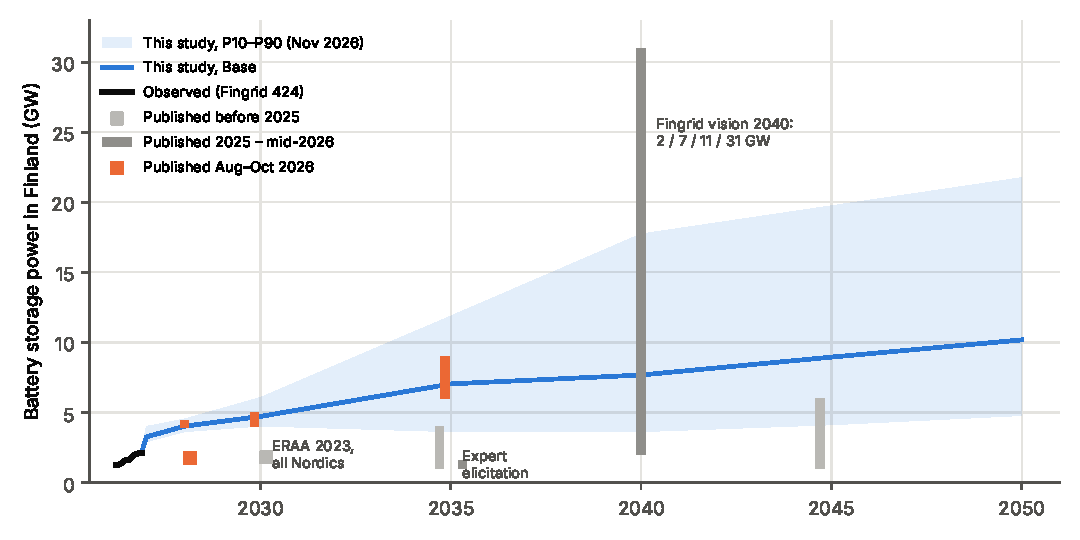
\includegraphics[width=\linewidth]{fig_vintages.pdf}
\caption{Finnish battery storage forecasts by publication date against the observed fleet and the pooled states of this study. Bars show published ranges and squares single values; the ERAA 2023 value covers all the Nordic countries.}
\label{fig:vintages}
\end{figure}

Finland is also an outlier in the global context (Table~\ref{tab:regions}).
At \val{pc-finland}\,kW per person, its fleet is two and a half to three times as dense as those of the United States (\val{pc-united}, utility scale) and China (\val{pc-china}), and six to seven times the world average (\val{pc-world}). Only Lithuania (\val{pc-lithuania}) is comparable; both are small power systems in which batteries have been built mainly for reserves and system services.
In 2050 the Base of this study corresponds to \val{pc-fi-2050}\,kW per person (\val{pc-fi-2050-low}--\val{pc-fi-2050-high}), against about 0.4 for the world in BloombergNEF's and IRENA's outlooks, 1.13 for Denmark and 0.8--0.9 for Sweden.
The economic method alone gives \val{pc-fi-2050-m3}\,kW per person.
A Finnish fleet several times denser than the global average is consistent with Finland's position today, but it is a strong assumption that the Base keeps Finland about two-thirds above its Danish neighbour, and the Low state, near the Nordic peers, should be read with that in mind.
Global outlooks therefore set the direction of technology and its cost for a Finnish study, but not Finnish volume, which is decided by the domestic revenue pool.

\begin{table}[t]
\centering
\caption{Installed battery storage per person and typical duration: Finland and other regions now, and in 2050 outlooks. Populations are approximate.}
\label{tab:regions}
\small
\begin{tabularx}{\linewidth}{@{}>{\raggedright\arraybackslash}X l r l >{\raggedright\arraybackslash}p{3.8cm}@{}}
\toprule
Region & When & GW & kW per person & Duration (h)\\
\midrule
\tabinput{generated/tab_regions.tex}
\bottomrule
\end{tabularx}
\par\footnotesize Sources: \citet{fingrid424}; Litgrid; US EIA; Terna; \citet{cnesa2026white}; Aurora; \citet{bnef2026neo,irena2024weto,dea2025af25,svk2026lma}; world stock estimated from BloombergNEF 2025 additions and its 2026 forecast.
\end{table}

\subsection{Revenue: reserves saturate, balancing grows, arbitrage covers part of the cost}\label{sec:markets}
Table~\ref{tab:market} and Figure~\ref{fig:reserves} summarise the Finnish revenue base.
Mean hourly capacity prices fell in every reserve product between 2023 and 2026, as procured volumes and battery participation grew \citep{nordictsos2025batteries,fingrid2026reserveday}, and the procurement cost of the hourly markets fell from \val{respool-2023} to an annualised \val{respool-2026}\,M\EUR.
Balancing energy, valued as the activated volume times its premium over the day-ahead price, partly offset the decline: the mFRR energy pool peaked at \val{mfrrpool-2025}\,M\EUR{} in 2025 and was \val{mfrrpool-2026}\,M\EUR{} in 2026 on an annualised basis.
Including aFRR energy, the combined flexibility pool was \val{totpool-2023}, \val{totpool-2024}, \val{totpool-2025} and \val{totpool-2026}\,M\EUR{} in 2023--2026, so it roughly halved in the year in which the fleet doubled.

Day-ahead arbitrage was evaluated with a perfect-foresight linear programme solved separately for each Helsinki delivery day, for a 1\,MW unit with a round-trip efficiency of 0.85 and a depth of discharge of 0.9, on hourly prices until 30 September 2025 and 15-minute prices thereafter. The central 2026 cost of cell wear enters the programme as a dispatch hurdle, so that the unit does not cycle for spreads too thin to justify its wear, but it is not deducted from the reported margin: augmentation and capital recovery over the economic life already pay for the wear, and deducting it again would count it twice. Margins are therefore net of charging cost and gross of wear.
In 2026 it earned \val{da-2-2026}\,k\EUR/MW at 2\,h and \val{da-4-2026}\,k\EUR/MW at 4\,h, against annualised costs of \val{ann-2-2026} and \val{ann-4-2026}\,k\EUR/MW (Figure~\ref{fig:arbitrage}).
Margins rise much less than proportionally with duration. The means for 2024--2026 are \val{dam-1}, \val{dam-2}, \val{dam-4} and \val{dam-8}\,k\EUR/MW at 1, 2, 4 and 8\,h, because Finnish daily price shapes have one or two deep troughs rather than long multi-hour plateaus.

A first-order free-entry check gives a sense of scale before the full model.
If the 2026 market is held fixed, batteries capture 85\,\% of the perfect-foresight margin and a share $s$ of the 2026 pool, and the fleet stops growing where revenue per MW meets cost, then at central cost the supportable fleet of 2\,h systems is \val{sf-2-2026-half}--\val{sf-2-2026-full}\,GW for $s$ between one half and one, rising to \val{sf-2-2030-half}--\val{sf-2-2030-full}\,GW with 2030 costs. For 4\,h systems the corresponding ranges are \val{sf-4-2026-half}--\val{sf-4-2026-full} and \val{sf-4-2030-half}--\val{sf-4-2030-full}\,GW.
With 2035 costs the captured day-ahead margin of a 4\,h system in today's market exceeds its annualised cost, so a fixed market no longer bounds the fleet at all; only the fleet's own effect on prices does.
The 2026 range brackets the installed fleet. The check leans high, because it ignores the erosion of day-ahead spreads by the fleet itself; the equilibrium of Section~\ref{sec:m3} replaces the fixed market with one that responds to the fleet and to demand.

\begin{table}[t]
\centering
\caption{Finnish flexibility revenue pools (M\EUR/yr) and perfect-foresight day-ahead arbitrage margin (k\EUR/MW/yr), with the margin as a share of 2026 annualised cost.}
\label{tab:market}
\small
\begin{threeparttable}
\begin{tabular}{@{}lrrrrrrrrr@{}}
\toprule
 & \multicolumn{4}{c}{Pools (M\EUR/yr)} & \multicolumn{4}{c}{DA margin (k\EUR/MW/yr)} & Margin/\\
\cmidrule(lr){2-5}\cmidrule(lr){6-9}
Year & Reserve cap. & mFRR en. & aFRR en. & Total & 1\,h & 2\,h & 4\,h & 8\,h & cost (\%)\\
\midrule
\tabinput{generated/tab_market.tex}
\bottomrule
\end{tabular}
\begin{tablenotes}\footnotesize
\item[a] 2026 to 14 November (\val{res-hours-2026} days), annualised. Reserve capacity covers the hourly markets for FCR-N, FCR-D up and down, aFRR up and down and mFRR up; Fingrid's yearly markets, FFR and weekly mFRR are excluded. Total reserve procurement in 2025 was 172\,M\EUR{} \citep{fingrid2026reserveday}.
\end{tablenotes}
\end{threeparttable}
\end{table}

\begin{figure}[t]
\centering
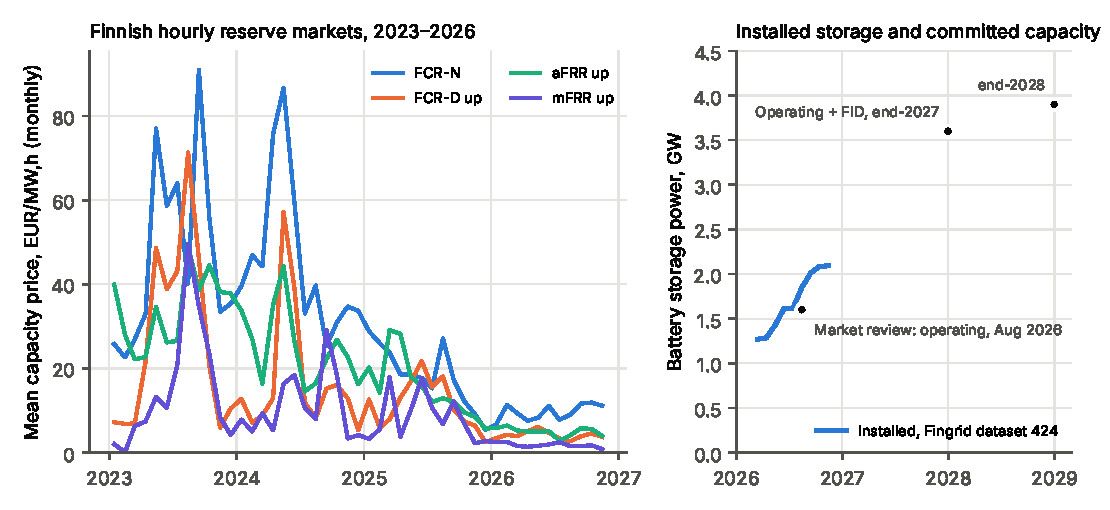
\includegraphics[width=\linewidth]{fig_reserves.pdf}
\caption{Monthly mean capacity prices in the Finnish hourly reserve markets (left), and installed storage power with the operating and committed capacity stated in the 2026 market review (right) \citep{fingridopendata,fingrid424,merilehto2026blog}.}
\label{fig:reserves}
\end{figure}

\begin{figure}[t]
\centering
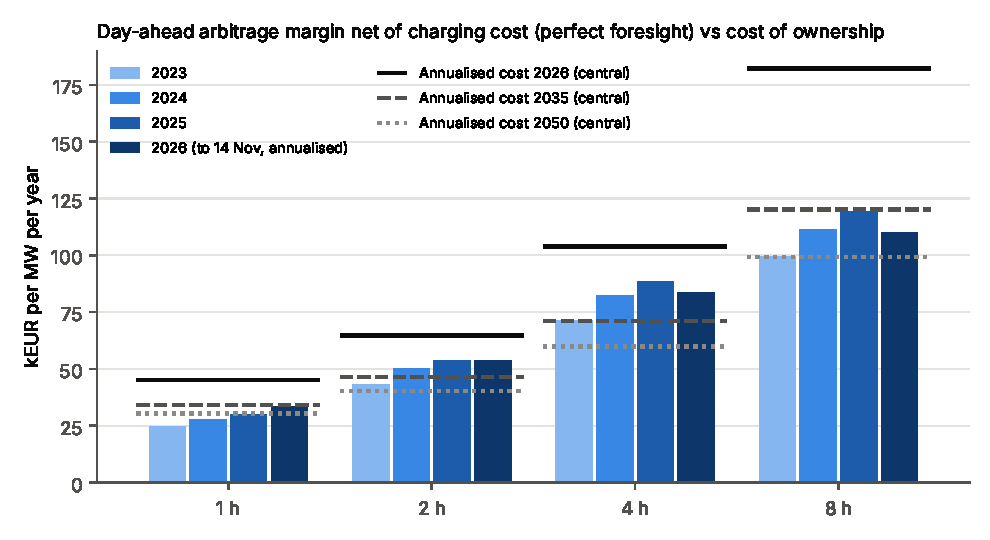
\includegraphics[width=0.85\linewidth]{fig_arbitrage.pdf}
\caption{Perfect-foresight day-ahead arbitrage margin by duration, 2023--2026, against the central annualised cost of ownership in 2026, 2035 and 2050.}
\label{fig:arbitrage}
\end{figure}

% =====================================================================
\section{Technology and cost}\label{sec:techcost}

This section treats Finland as what it is technologically: a buyer of globally traded battery equipment, mostly of Chinese origin, assembled into projects through a European supply chain of integrators, contractors and grid connections, and financed at a Finnish cost of capital.
The cost model is built on that distinction. It separates four sources of cost uncertainty, global technology learning, the European premium, financing and domestic project costs, so that the influence of each on the fleet can be measured on its own (Section~\ref{sec:sobol}).

\subsection{Technology landscape and performance}\label{sec:tech}
Through the 2030s the Finnish storage question is a lithium-ion question.
Lithium iron phosphate (LFP) chemistry accounts for practically the whole Finnish fleet. Stationary cells moved from the 280--314\,Ah class to 500--690\,Ah in 2024--2026, and a standard 20-foot container now holds 6.25\,MWh \citep{essnews2026bigcells,esn2024tener}.
Sodium-ion is the plausible chemistry hedge for Finland. It is expected to be 20--30\,\% cheaper than LFP at scale and its manufacturers claim operation down to $-40$\,$^\circ$C, but independent tests find that its internal resistance rises far faster than LFP's in the cold and that conventional cells barely recharge below $-10$\,$^\circ$C. It is therefore treated as a cost and cold-start option for the 2030s, carried by the low-cost case, rather than as the base chemistry.
Among long-duration options, pumped hydro is the only multi-day electricity storage with Finnish projects: Kemijoki's Ailangantunturi plant of 550\,MW, planned for operation around 2033 subject to an investment decision, and Pohjolan Voima's PUHTI of about 500\,MW and 25\,GWh \citep{kemijoki2026ailanga,pvo2025puhti}.
Iron-air storage would cross the cost threshold that \citet{sepulveda2021ldes} identify for system value if its targets are met, but it has no Finnish project and is not modelled; neither are vanadium flow, compressed air and gravity storage.
Thermal storage and hydrogen compete with batteries for the same low-price hours but return no electricity, and they enter only as competing flexibility.

Manufacturers' terms have moved ahead of the assumptions used by agencies.
Tesla's Megapack~3 is offered with at least 10\,000 cycles, up to 25 years of design life and up to 20 years of warranty, and Fluence guarantees a 25-year system life under its service plans, whereas NREL's technology baseline still assumes a 15-year life with augmentation financed through fixed operating cost \citep{nrel2025batterycost}. PNNL's baseline for LFP warranties is 10--15 years or 10\,000 cycles at 80\,\% depth of discharge \citep{viswanathan2022pnnl}.
Field data temper the vendor claims. Independent measurements of German home systems and of an Italian 7.4\,MW market-trading plant both find capacity losses of about 2--3\,\% a year, and US operators report 20--30\,\% over the first decade.
The Danish Energy Agency's technology data, updated for lithium-ion batteries in May 2025, point the same way, with a technical lifetime rising from 15 years in 2025 to 20 in 2030 and 25--30 thereafter, cycle life rising from 5\,000 to 20\,000 by 2050, and an AC round-trip efficiency of 91--92\,\% before standby losses \citep{dea2025techdata}.
The model therefore uses an economic life of 20 years (15--25), cycle life that rises from 8\,000 full cycles for a 2025 vintage (6\,000--12\,000) to 12\,000 in 2035 and 15\,000 in 2050, and an augmentation allowance, as an initial overbuild or as later additions, of 15\,\% of the energy equipment in 2025 falling to 5\,\% in 2050.
Round-trip efficiency, measured as AC at the grid connection and excluding auxiliaries, starts at 0.85 in 2025 (0.82--0.89) and rises by 2 percentage points by 2035 and 3 by 2050, following PNNL's transformer-level trajectory, NREL's 85\,\% and Lazard's 86--92\,\% \citep{viswanathan2022pnnl,nrel2025batterycost,lazard2026lcoe}.

Auxiliary consumption for heating, cooling and control is the least measured parameter for a Nordic fleet.
A design figure of more than 15\,MWh per MWh of capacity per year \citep{esn2026enertis} corresponds to about 1.7\,kW/MWh; an air-cooled Italian plant measured 3.3\,kW/MWh (a secondary reading of \citealt{dimovski2026aux}); and manufacturer figures for liquid-cooled 5\,MWh blocks in cold weather correspond to 2.2--4.4\,kW/MWh. No Nordic field measurement was found.
The model uses \val{aux-2025}\,kW/MWh for a 2025 vintage (0.9--3.3), falling to \val{aux-2050}\,kW/MWh by 2050 as thermal design improves.

Grid-forming obligations add a component that does not depend on market revenue.
Since October 2026, new large wind and solar plants on weak grid connections must provide grid-forming support, for example with batteries of 10--30\,\% of plant capacity \citep{essnews2026gridforming}, and ENTSO-E's proposal for the next generator code would require grid-forming capability from all new storage above 1\,MW \citep{essnews2025rfg}.
The model adds 0, 0.8 or 3.0\,GW of such units by 2050. They are counted in the stock at 1\,h, and they compete with market batteries at half weight because they may trade only while their stabilising capability is preserved.

\subsection{Prices in Finland, Europe and the rest of the world}\label{sec:prices}
Battery prices diverged sharply by region in 2024--2026 (Table~\ref{tab:prices}).
In BloombergNEF's 2025 survey of turnkey systems, which excludes construction and grid connection, the global average fell 31\,\% to 117\,USD/kWh. China averaged 73\,USD/kWh, Europe 177 and the United States 219 \citep{bnef2025ess}.
A year earlier Europe had stood at 275\,USD/kWh against China's 101, so Europe's premium over China narrowed from about 2.7 to 2.4 times in a single year.
Chinese prices then rebounded in 2026, by 10--25\,\% for awarded systems, as lithium carbonate more than doubled from its 2025 low and the Chinese export rebate on batteries was cut from 13\,\% to 6\,\%, with its removal scheduled for January 2027.

The European premium is not a hardware premium.
Chinese DC blocks bound for Europe were priced at 71--89\,USD/kWh free on board in mid-2026, about the same as Chinese domestic systems, and the EU import duty on lithium-ion accumulators is at most 2.7\,\% with no trade-defence duty on stationary batteries.
What separates equipment at Chinese prices from a European turnkey price is integration, warranty risk, compliance with European grid, fire and cyber requirements, engineering and the small size of many projects.
Large European auctions show how far this premium can be compressed: Italy's MACSE auction cleared 10\,GWh at prices that Ember translates into about 120\,USD/kWh all-in, and Ember's benchmark for large 4\,h projects outside China and the United States is 125\,USD/kWh, of which about 75 is equipment and 50 installation and grid connection \citep{ember2025cheap}.
Disclosed Nordic and Baltic projects sit well above these levels: a 30\,MW and 66\,MWh order placed in Finland in 2025 works out at about 258\,\EUR/kWh, and Estonian and Latvian 2\,h plants contracted in 2023--2024 at about 370 and 480\,\EUR/kWh including substations. German investment cases for 2026 imply 234\,\EUR/kWh for 4\,h and 350 for 2\,h.

Finland therefore participates fully in the global market for battery equipment but only partly in the global market for battery projects.
The model's 2025 anchor for a 4\,h system, about 207\,\EUR/kWh all-in before augmentation, sits at the level of Australia's official estimate (about 216), below German and US levels, and at roughly twice the price floor set by the largest auctions. Its fit to the two disclosed Finnish contracts (Section~\ref{sec:cost}) supports it for today's small and short Finnish projects.

\begin{table}[t]
\centering
\caption{Stationary battery cost levels by market and scope (EUR/kWh, converted at 1.08, 1.13 and 1.16\,USD/EUR for 2024--2026). Turnkey excludes construction and grid connection; all-in includes both.}
\label{tab:prices}
\footnotesize
\begin{tabular}{@{}llrrrr@{}}
\toprule
Market & Scope & 2024 & 2025 & 2026 & 2035 outlook\\
\midrule
China & Turnkey (BNEF) & 94 & 65 & -- & 36\\
China & Awarded AC systems, 4\,h & -- & 59 & 66--76 & --\\
China & Construction (EPC), 4\,h & -- & 119 & 107--117 & --\\
Europe & Turnkey (BNEF) & 255 & 157 & -- & 89\\
Italy & MACSE auction, implied all-in 4\,h+ & -- & $\sim$106 & -- & --\\
Outside China and US & All-in 4\,h+ (Ember) & -- & 111 & -- & --\\
Germany & All-in, 4\,h / 2\,h & -- & -- & 234 / 350 & --\\
Finland & Integrator order, 2.2\,h & -- & $\sim$258 & -- & --\\
Estonia / Latvia & All-in incl. substation, 2\,h & -- & 369 / 482 & -- & --\\
Australia & All-in 4\,h (CSIRO GenCost) & -- & $\sim$216 & -- & --\\
United States & Turnkey (BNEF) & 219 & 194 & -- & 96\\
United States & All-in 4\,h (NREL) & 309 & 297 & -- & 225 (mid)\\
\midrule
Finland, this study & All-in 4\,h incl. augmentation & -- & \val{capex-4-2026}$^{a}$ & -- & \val{capex-4-2035}\\
\bottomrule
\end{tabular}
\par\footnotesize $^{a}$ 2026 value. Sources: \citet{bnef2025ess,ember2025cheap,nrel2025batterycost}; CNESA and EnergyTrend tender data; Terna (MACSE); Modo Energy (Germany); CSIRO GenCost 2025-26; trade-press reports of disclosed contracts.
\end{table}

\subsection{Cost model}\label{sec:cost}
Installed capital cost per kW of a system of duration $d$ hours built in year $t$ is
\begin{equation}\label{eq:capex}
K(d,t) = c_E(t)\,d\,\bigl(1+\alpha(t)\bigr) + c_P(t) + b\,K_0(d)\,(1+g)^{t-2025} + G,
\end{equation}
where $c_E$ and $c_P$ are the energy- and power-related equipment costs, $\alpha$ the augmentation allowance, $b\,K_0(d)$ installation and construction at 15\,\% of the 2025 equipment cost, declining by $g$ of 0--2\,\% a year in real terms, and $G$ the grid connection of 150\,\EUR/kW (100--250), which is held flat in real terms.
The 2025 equipment costs are anchored on BloombergNEF's turnkey prices. Solving its global prices of 124\,USD/kWh at 2\,h and 110 at 4\,h for the two components and scaling them by the ratio of European to global prices gives $c_E=\val{cE}$\,\EUR/kWh and $c_P=\val{cP}$\,\EUR/kW \citep{bnef2025ess}.

The equipment costs are then split by what drives their learning:
\begin{equation}\label{eq:components}
\begin{aligned}
c_E(t) &= \underbrace{\max\!\bigl(f,\; c_{\mathrm{cell},0}(1-\lambda_c)^{D_{\mathrm{Li}}(t)}\bigr)}_{\text{cells}}
 + \underbrace{c_{\mathrm{frt}}}_{\text{freight, duty}}
 + \underbrace{c_{\mathrm{bos},0}(1-\lambda_b)^{D_{\mathrm{st}}(t)}}_{\text{DC balance of system}}
 + \underbrace{\pi(t)}_{\text{European premium}},\\
c_P(t) &= c_{P,0}(1-\lambda_b)^{D_{\mathrm{st}}(t)}.
\end{aligned}
\end{equation}
Cells, at \val{comp-cells-2025}\,\EUR/kWh ex works China in 2025, learn at $\lambda_c=18\,\%$ (15--21\,\%) per doubling of cumulative global lithium-ion production $D_{\mathrm{Li}}$, down to a materials floor $f$ of 18\,\EUR/kWh (12--28). The learning rate is the long-run record for lithium-ion cells, 18.9--20.4\,\% per doubling for 1992--2016 with no detectable slowdown \citep{ziegler2021rates}; empirically grounded forecasts of this kind have been well calibrated in back-tests up to twenty years ahead \citep{way2022empirical}.
Cumulative production stood at about 4.7\,TWh at the end of 2025, and IEA-type demand outlooks imply 3.0--3.7 further doublings by 2035 and 4.65--5.6 by 2050 (central 3.3 and 5.1).
DC balance of system (\val{comp-dcbos-2025}\,\EUR/kWh: racks, battery management, thermal systems and enclosures) and power conversion learn at $\lambda_b=12\,\%$ (8--15\,\%) per doubling of cumulative stationary deployment $D_{\mathrm{st}}$, between the 8--12\,\% implied by NREL's component projections and the 16\,\% that \citet{schmidt2017experience} measured for utility systems as a whole.
The European premium $\pi$, the residual \val{comp-premium-2025}\,\EUR/kWh or \val{prem-share-2025}\,\% of the 2025 energy cost, declines by 5\,\% a year to 2035 and 2\,\% a year thereafter, which reproduces the narrowing of the Europe--China gap implied by BloombergNEF's 2035 outlook. Its slow case declines at 2\,\% and 1\,\% a year, its fast case at 10\,\% and 3\,\%.
For 2026 and 2027 the equipment index follows the observed rebound (1.00 and 0.97 of the 2025 level in the central case, up to 1.10 in the high case) and rejoins the learning path by 2030. The rebound is applied to the traded hardware only, so the European premium keeps its own convergence path through these years.
The high-cost case adds a lithium premium to cell cost that rises to 20\,\% around 2030 and fades by 2035, representing a renewed raw-material squeeze of the kind seen in 2021--2022 and 2026; it is the reason the high case is flat rather than falling in the late 2020s.

The learning of globally traded components and the convergence of the European premium are separate uncertainties in the model.
The first represents global technology development, in which Finland shares fully; the second represents how quickly the European and Finnish project market comes to resemble the global one.
Calibrated this way, the central case reproduces BloombergNEF's 2035 forecast of 101\,USD/kWh for a European 4\,h turnkey system to within 1\,\% (the code asserts agreement within 3\,\%).

The model reproduces two disclosed Finnish contracts, excluding grid connection.
For Mertaniemi (38\,MW and 43\,MWh, contracted in 2024) it gives \val{val-mert-model}\,\EUR/kW against \val{val-mert-obs} observed, a ratio of \val{val-mert-ratio}. For Tervola (20\,MW and 41\,MWh, ordered in 2026 for ``over 8\,M\EUR{}'' including services) it gives \val{val-terv-model} against at least \val{val-terv-obs}\,\EUR/kW, a ratio of \val{val-terv-ratio}.
The annualised cost of ownership adds capital recovery over the economic life, fixed operation and maintenance as a share of equipment and installation cost, Fingrid's storage capacity fee of 1.137\,\EUR/kW per year, and auxiliary electricity.

Four independent uncertainty dimensions span the cost of a Finnish project.
\emph{Technology learning} moves the learning rates, doublings and materials floor of the globally traded components in Equation~\eqref{eq:components}.
The \emph{European premium} moves the rate at which $\pi$ converges.
\emph{Financing} moves the real cost of capital (5, 7 and 10\,\%) together with the economic life (25, 20 and 15 years), since lenders price both the same risks.
\emph{Domestic project costs} move grid connection (100, 150 and 250\,\EUR/kW), the decline of installation cost (2, 1 and 0\,\% a year), fixed operation and maintenance (1, 2 and 3\,\%) and auxiliary load together.
Annualised cost is computed on the grid of the three cases of each dimension and interpolated log-linearly for each Monte Carlo draw. Earlier versions bundled all four into a single uncertainty, which attributed to technology what is really a matter of finance and local cost.

The marginal cost of a cycle is
\begin{equation}\label{eq:cycle}
c_{\mathrm{cyc}} = \frac{C_{\mathrm{repl}}}{N\cdot \mathrm{DoD}} + \Bigl(\frac{1}{\eta}-1\Bigr)p_{\mathrm{ch}},
\end{equation}
where $C_{\mathrm{repl}}$ is the replacement cost of the battery blocks (70\,\EUR/kWh in 2025, following $c_E$), $N$ the cycle life, $\eta$ the round-trip efficiency and $p_{\mathrm{ch}}$ the average charging price (central 45\,\EUR/MWh).
It serves only as the hurdle in the dispatch programme, not as a cost deducted from margins (Section~\ref{sec:markets}). It is \val{cyc-2025}\,\EUR/MWh in 2025, inside the market review's 15--30\,\EUR/MWh, and the low and high parameter cases (\val{cyc-2025-low}--\val{cyc-2025-high}) bracket that range. It falls to \val{cyc-2035}\,\EUR/MWh in 2035 and \val{cyc-2050} in 2050, by which time the efficiency-loss term, which does not learn, has become the larger part (Figure~\ref{fig:capex}).

\begin{table}[t]
\centering
\caption{Component cost model, central case (EUR2025). Energy components in EUR/kWh, power conversion in EUR/kW; 4\,h turnkey is $c_E + c_P/4$; the index is relative to 2025 with the low--high range; all-in includes installation, augmentation and grid connection.}
\label{tab:components}
\small
\begin{tabular}{@{}lrrrrrrrcc@{}}
\toprule
Year & Cells & Freight & DC BOS & Premium & $c_E$ & $c_P$ & 4\,h turnkey & Index & 4\,h all-in\\
\midrule
\tabinput{generated/tab_components.tex}
\bottomrule
\end{tabular}
\end{table}

\begin{table}[t]
\centering
\caption{Central cost paths: installed capex per kWh including grid connection by duration, low--high range for 4\,h, annualised cost of ownership per kW, and 4\,h levelised cost of storage excluding charging energy at 250 cycles per year.}
\label{tab:cost}
\small
\begin{tabular}{@{}lrrrrcrrrrr@{}}
\toprule
 & \multicolumn{4}{c}{Capex (\EUR/kWh)} & 4\,h low--high & \multicolumn{4}{c}{Annualised (k\EUR/MW/yr)} & LCOS 4\,h\\
\cmidrule(lr){2-5}\cmidrule(lr){7-10}
Year & 1\,h & 2\,h & 4\,h & 8\,h & (\EUR/kWh) & 1\,h & 2\,h & 4\,h & 8\,h & (\EUR/MWh)\\
\midrule
\tabinput{generated/tab_cost.tex}
\bottomrule
\end{tabular}
\end{table}

\begin{figure}[t]
\centering
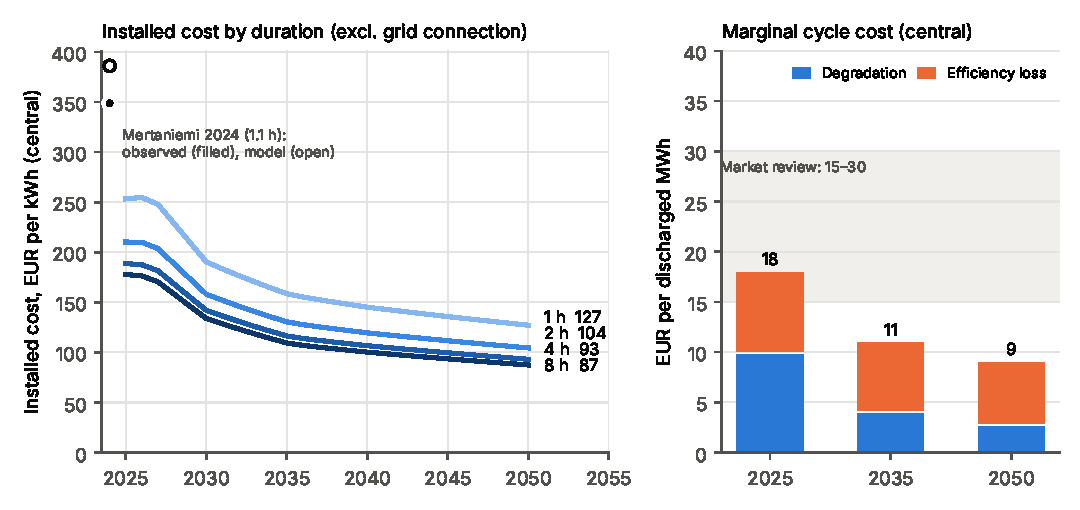
\includegraphics[width=\linewidth]{fig_capex_cycle.pdf}
\caption{Installed cost per kWh by duration with the Mertaniemi contract (left), and marginal cycle cost split into degradation and efficiency loss, against the 15--30\,\EUR/MWh range of the 2026 market review (right).}
\label{fig:capex}
\end{figure}

\subsection{Is the cost path too slow?}\label{sec:howfast}
Table~\ref{tab:components} and Figure~\ref{fig:costcompare} answer this question in two parts.
For the most global part of a battery system, the cells, the path is fast. Their cost falls to \val{comp-cells-2035}\,\EUR/kWh by 2035 and reaches the materials floor in the late 2030s; a single Wright's-law index for cells alone gives \val{idxB-2035} in 2035 and \val{idxB-2050} in 2050.
For a complete European system the central equipment index is slower, \val{idxC-central-2035} in 2035 and \val{idxC-central-2050} in 2050, because cells are only about a quarter of a European turnkey price in 2025 and the rest learns more slowly.
This central path is almost identical to the one obtained by chaining BloombergNEF's 2035 forecast with NREL's mid-case ratio to 2050 (\val{idxA-2035} and \val{idxA-2050}), and it lies between NREL's low and mid cases. Against the Nordic official source it is faster, not slower. The Danish Energy Agency's May 2025 data imply a 4\,h index of only 0.76 in 2035 and 0.72 in 2050, at a level of about 320\,\EUR/kWh in 2025 excluding the transmission connection \citep{dea2025techdata}. The reason is that the Danish reference is a single 3\,MWh container, for which construction, cabling and contractor work make up more than half the cost and fall by only a fifth to 2050; the Danish battery component alone falls by 42\,\% to 2035 and then flattens, much like the cells and DC components of this model. The older Danish curve of 2018--2019, which most European models still use, starts higher but falls faster.
In absolute terms, the central 4\,h all-in cost falls from \val{capex-4-2026}\,\EUR/kWh in 2026 to \val{capex-4-2035} in 2035 and \val{capex-4-2050} in 2050.

\begin{figure}[t]
\centering
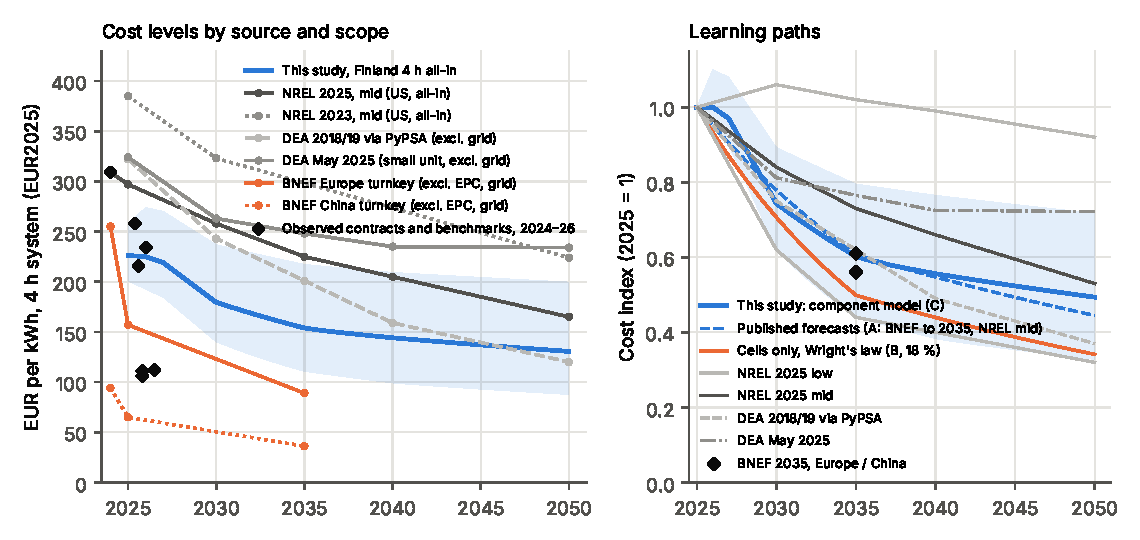
\includegraphics[width=\linewidth]{fig_cost_compare.pdf}
\caption{Left: 4\,h cost levels of this study (band: low--high) against other projections and observed prices; scopes differ as labelled. Right: learning paths as indices of each source's own base year. Sources: \citet{nrel2025batterycost,bnef2025ess,ember2025cheap,dea2025techdata}; the older Danish data as compiled by PyPSA; observed values as in Table~\ref{tab:prices}.}
\label{fig:costcompare}
\end{figure}

The record of past forecasts points the same way as the comparison (Table~\ref{tab:trackrecord}).
Survey-based near-term forecasts of battery prices have been roughly unbiased: six BloombergNEF pack-price forecasts made in 2019--2024 for one to five years ahead have a mean ratio of forecast to outcome of about 1.04, too optimistic during the lithium spike of 2021--2022 and too pessimistic during the price fall of 2023--2025.
Long-horizon institutional and academic projections, by contrast, have consistently been too high. NREL's 2023 mid case for 2025 was about 1.3 times the outcome, and NREL now describes its new costs as closest to its earlier low case \citep{nrel2025batterycost}. The system cost that \citet{schmidt2017experience} projected for the point at which 1\,TWh of storage had been installed was about 2.6--2.8 times what was realised. \citet{way2022empirical} find that energy-model projections for solar, wind and batteries have systematically underestimated deployment and overestimated costs.
Deployment forecasts have been even further off. BloombergNEF's 2017 forecast of 305\,GWh of storage worldwide by 2030 was matched by installations in 2025 alone, and in Finland every forecast published before 2025 has already been overtaken by the observed fleet (Section~\ref{sec:external}).

Three conclusions follow for the model.
First, a central path anchored on survey forecasts to 2035 is consistent with the record, but the slower decline after 2035 is a property of Wright's law, not a pessimistic choice: about three doublings of global production fall in 2025--2035 and fewer than two in 2035--2050.
Second, the tails should not be set wider than the record allows. A case with practically no learning to 2050, which would leave a 4\,h system near 280\,\EUR/kWh, has no precedent in more than thirty years of lithium-ion data, so the high-cost case keeps 4\,h systems at about \val{capex-4-high-2050}\,\EUR/kWh in 2050, while the low-cost case reaches \val{capex-4-low-2050}.
Third, the European premium is a genuine and separate uncertainty. If it converged fast, the 2035 equipment index would be \val{idxC-premlow-2035} rather than \val{idxC-central-2035}; if it stayed sticky, \val{idxC-premhigh-2035}. Trade policy, not technology, is the credible route to a flat European cost path, as the United States illustrates, where tariffs and restrictions on Chinese cells have kept costs about a quarter above Europe's.

A natural further question is whether the outlook depends on a chemistry superior to lithium-ion. It does not. The central path assumes only continued learning of LFP cells down to a materials floor, and two stress cases test what a better technology would add (Section~\ref{sec:stress}). A post-lithium chemistry that halves cell cost from 2030, with 50\,\% longer cycle life, higher efficiency and 40\,\% lower auxiliary consumption, raises the central equilibrium from \val{stress-central-gw-2035} to \val{stress-postlithiumchemistrycells50from2030andbetterperformance-gw-2035}\,GW in 2035 and from \val{stress-central-gw-2050} to \val{stress-postlithiumchemistrycells50from2030andbetterperformance-gw-2050}\,GW in 2050. Even the bound in which cells cost nothing from 2030 gives only \val{stress-boundcellsfreeofchargefrom2030-gw-2035} and \val{stress-boundcellsfreeofchargefrom2030-gw-2050}\,GW. Longer cycle life adds nothing in this case, because at one or two cycles a day the calendar life, not the cycle life, ends a Finnish battery's economic life; the gain comes from cheaper cells, higher efficiency and lower auxiliary load. Because cells are a small and shrinking share of a Finnish project's annualised cost, a cheaper chemistry moves the fleet less than cheap capital (\val{stress-cheapcapital-gw-2050}\,GW in 2050) or weaker cannibalisation does, and less than grid connection at 100 instead of 150\,\EUR/kW (\val{stress-lowdomesticprojectcosts-gw-2050}\,GW). Superior technology would matter for a different question, multi-day storage for cold and windless periods, where iron-air or other long-duration technologies rather than cheaper lithium-ion cells would be needed; that question lies outside the estimand of this paper.

\begin{table}[t]
\centering
\caption{Track record of battery cost and deployment forecasts (ratio of forecast to outcome; above 1 means too pessimistic on cost or too optimistic on deployment).}
\label{tab:trackrecord}
\footnotesize
\setlength{\tabcolsep}{4pt}
\begin{tabularx}{\linewidth}{@{}>{\raggedright\arraybackslash}X >{\raggedright\arraybackslash}p{2.8cm} >{\raggedright\arraybackslash}p{2.3cm} >{\raggedright\arraybackslash}p{2.4cm} >{\raggedright\arraybackslash}p{1.8cm}@{}}
\toprule
Forecast (vintage) & Quantity, target year & Forecast & Outcome & Ratio\\
\midrule
BloombergNEF pack survey (2019) & Average pack, 2023 & $\sim$100\,USD/kWh & 139 & 0.72 (real $\sim$0.86)\\
BloombergNEF (2021) & Average pack, 2022 & 135\,USD/kWh & 151 & 0.89\\
BloombergNEF (2022) & Average pack, 2023 & 152\,USD/kWh & 139 & 1.09\\
BloombergNEF (2023) & Average pack, 2024 / 2025 & 133 / 113\,USD/kWh & 115 / 108 & 1.16 / 1.05\\
BloombergNEF (2023) & All-segment pack, 2030 & 80\,USD/kWh & stationary 70 in 2025 & beaten 5 yr early\\
NREL cost projections (2023, mid) & US 4\,h installed, 2025 & $\sim$416\,USD/kWh (2024\$) & 321 & 1.30 (low case 1.03)\\
\citet{schmidt2017experience} & System at 1\,TWh installed & 325\,$\pm$\,125 USD/kWh & 110--125 (2025) & 2.6--2.8\\
BloombergNEF (2017) & Global storage, 2030 & 305\,GWh cumulative & 307\,GWh added in 2025 & $\ll$\,1\\
BloombergNEF (2025) & Global additions, 2025 & 247\,GWh & 307\,GWh & 0.80\\
US EIA AEO2022 & US batteries, 2050 & 28\,GW & $\sim$52\,GW in mid-2026 & $<$\,0.55\\
ENTSO-E ERAA 2023 & Nordic batteries, 2030 & $\sim$1.8\,GW & Finland alone 2.09\,GW (2026) & $<$\,0.9\\
\bottomrule
\end{tabularx}
\par\footnotesize Sources: BloombergNEF annual battery price survey releases 2019--2025; \citet{nrel2025batterycost} and its 2023 predecessor; \citet{schmidt2017experience}; \citet{bnef2026hundred}; US EIA; Nordic Energy Research on ERAA 2023; \citet{fingrid424}.
\end{table}

% =====================================================================
\section{Forecast methods}\label{sec:methods}

Each method returns a joint Monte Carlo sample of power and energy for every year, with \val{ndraws} draws per method from a fixed seed (\val{seed}).
Three rules apply to all of them.
A method enters the pool only at the checkpoints where it carries information of its own. The queue method (M1) is pooled to 2030, the top-down method (M4) from 2035, and the other three throughout, so the set of methods is constant from 2035 and the state paths do not jump when a method drops out.
No draw may lie below the stock that already exists or is under construction. This floor is today's fleet plus 85\,\% of the FID tranche, with Weibull survival, and it is \val{floor-2028}\,GW in 2028, \val{floor-2035}\,GW in 2035 and \val{floor-2040}\,GW in 2040.
Power and energy stay paired within each draw, so that the distribution of energy reflects the power distribution and the duration assumptions jointly.

\subsection{M1: project queue}
The queue is divided into three stages, each with a triangular realisation probability and a spread of commercial operation dates. Projects with an investment decision that are not yet operating amount to 1.808\,GW at 2.8\,h, with a probability between 0.85 and 1 and operation in 2027 or 2028. Permitted projects net of these amount to 0.887\,GW, with a probability of 0.3--0.7 and operation in 2028--2030. Projects in early planning amount to 9.2\,GW at 3.0\,h, with a probability of 0.05--0.30 and operation in 2029--2032.
A Beta-distributed lumpiness factor reflects the fact that a few 125\,MW projects dominate each stage.
The market review's text implies that 83\,\% of the FID tranche would operate in 2027. With 25--30\,\% of capacity slipping by one year (\cls{a}), the weights used are 0.6 for 2027 and 0.4 for 2028.

\subsection{M2: logistic diffusion through two anchors}
The stock follows a logistic curve $N(t)=K/(1+e^{-z(t)})$ with $z$ linear in time. It passes through the observed stock $N(T_0)=\val{start-gw}$\,GW in November 2026 and, draw by draw, through M1's realised stock at the end of 2028, $N_{2028}$, which fixes the rate
\begin{equation}
r = \frac{\operatorname{logit}(N_{2028}/K)-\operatorname{logit}(N(T_0)/K)}{2029.0-T_0}.
\end{equation}
The saturation level $K$ is log-uniform between 4 and 31\,GW, that is, between Fingrid's 2030 Moderate state and the maximum of its 2040 vision, which also matches the volume of storage connection enquiries. In draws where $K$ would not exceed $N_{2028}$ the logistic cannot pass through both anchors, so $K$ is raised to $1.1\,N_{2028}$; this affects only draws in which M1 already reaches the lower part of the prior.
The implied time from 10\,\% to 90\,\% of saturation is \val{m2-dt-p10}--\val{m2-dt-p90} years (median \val{m2-dt-p50}), consistent with the fast diffusion of small, modular technologies \citep{wilson2020granular}.
Because the curve approaches $K$ by about 2038, M2's later checkpoints carry its saturation prior rather than dynamics, and the paper says so wherever M2 is pooled.

\subsection{M3: free-entry equilibrium}\label{sec:m3}
Revenue per MW of a battery of duration $d$ built in year $t$, in a fleet of $N$\,GW, is modelled as
\begin{equation}\label{eq:rev}
R_d(N,t) = \kappa\, \tilde m_d(t)\, F(t)^{\varepsilon_{\mathrm{flex}}\left(1+\tau\log_2(d/2)\right)}
\Bigl(\frac{N+N_x(t)}{N_0}\Bigr)^{-\varepsilon_{\mathrm{own}}}
+ \frac{e_d\, s\, P_0\, F(t)^{\varepsilon_{\mathrm{pool}}}}{N+N_x(t)}\Bigl(\frac{N+N_x(t)}{N_0}\Bigr)^{-\varepsilon_{\mathrm{sat}}}.
\end{equation}
The first term is arbitrage. The margin $\tilde m_d(t) = m_d + q_d\,\bar p_{\mathrm{ch}}\,(1/\eta_{2026} - 1/\eta(t))$ starts from the measured 2024--2026 day-ahead margin $m_d$ at the 2026 fleet $N_0$, net of charging cost but not of cell wear (Section~\ref{sec:markets}), and credits a vintage built in year $t$ with its higher round-trip efficiency $\eta(t)$ at the measured discharged energy $q_d$ and average charging price $\bar p_{\mathrm{ch}}$; holding dispatch fixed makes this a lower bound on the gain. $\kappa$ (0.75--0.95) is the share of the perfect-foresight margin captured in practice.
The flexibility-need index $F(t)$ is consumption growth, from 88\,TWh in 2026 to 110--162\,TWh in 2035 and 134--200\,TWh in 2050, multiplied by a VRE-share multiplier that reaches 1--1.6 by 2050.
The tilt $\tau$ (0--0.3) lets flexibility growth favour longer durations, standing in for the wider multi-hour spreads that more wind and solar would create.
$N_x$ is competing capacity, consisting of pumped hydro (0, 0.55 or 1.05\,GW from 2033 or 2036) and the grid-forming units at half weight.

The second term is the reserve and balancing pool. Its 2026 size is $P_0=124.7$\,M\EUR{}; it grows with flexibility need at elasticity $\varepsilon_{\mathrm{pool}}$, is shared by batteries and competing capacity, and shrinks as the flexible fleet grows at elasticity $\varepsilon_{\mathrm{sat}}$ (0.2--0.9). The last term reflects the evidence of Section~\ref{sec:markets}: the euro value of the pool did not stay fixed as batteries entered, but fell as they bid down clearing prices, so revenue per MW falls faster than $1/N$. Batteries capture a share $s$ (0.3--0.8) of the pool, and the eligibility factor $e_d$ is 0.4 for 1\,h systems, which cannot meet the endurance rules of all products, and 1 otherwise.

The cannibalisation elasticity $\varepsilon_{\mathrm{own}}$ (0.3--1.2, central 0.8) is anchored on \citet{savelli2026cannibalisation}, who find across European markets that a 10\,\% increase in battery capacity cuts battery profit by about 8\,\%. Spanish evidence that daily spreads halve at about 30\,GWh of storage \citep{seville2026spain} supports the same order of magnitude.
Cannibalisation is applied to fleet power, as the elasticity is estimated; because day-ahead spreads flatten with shifted energy rather than power, applying it to fleet energy is reported as a stress case (Section~\ref{sec:stress}).
The flexibility elasticity $\varepsilon_{\mathrm{flex}}$ (0.3--1.5) reflects the finding that more renewable capacity raises battery profit, although the benefit fades as storage grows \citep{savelli2026cannibalisation,dumitrescu2024price}. Its low end also covers the possibility that much of the new load is itself flexible (electric boilers, electrolysers) and compresses rather than widens spreads.

In each year the desired fleet $N^*_d$ solves $R_d(N^*_d,t)=A_d(t)$, where $A_d$ is the annualised cost of a new system interpolated log-linearly between the low, central and high cases of each of the four cost dimensions (technology learning, European premium, financing and domestic project costs), and the market builds the duration with the largest $N^*_d$.
The stock is tracked by vintage. No unit retires before a warranted minimum life of ten years; thereafter survival is Weibull (shape 3) with a mean life of 15 years for 2025 vintages, rising to 20 years by 2050. Additions are limited to 0.6--2.5\,GW per year and to a connection cap of 31\,GW, and the committed tranche is added in 2027--2028 regardless of the equilibrium.
The \val{m3-npar} uncertain parameters are sampled from triangular or uniform distributions (Appendix~\ref{app:params}).
With central parameters the equilibrium for 2026 is \val{m3c-nstar-2026}\,GW against \val{start-gw}\,GW installed, so a revenue model calibrated only on market data comes close to the observed fleet; the difference is consistent with the 3.9\,GW already committed for 2028.

\subsection{M4: top-down shares}
Half of M4's draws scale the global outlook and half use Nordic peers.
In the first sub-method the global battery fleet is drawn from the published range, 900--1\,200\,GW in 2030, 1\,400--2\,900\,GW in 2035 and 3\,800--4\,100\,GW in 2050 with 2040 interpolated \citep{iea2025weo,bnef2026neo,irena2024weto}, at the same quantile in every year. It is multiplied by a Finnish share that moves log-linearly from today's 0.46\,\% to 0.25--0.50\,\% in 2050.
In the second, Finland's stock moves log-linearly to the 2050 per-person level of a Nordic peer, either Denmark at 1.14\,kW per person or Sweden at 0.78--0.89\,kW per person (a secondary reading).
Scaling by population understates the peer benchmark for Finland, which uses about twice as much electricity per person as Denmark; scaling by present consumption instead gives about 16\,GW for the Danish peer. Because that alternative compares 2050 peer capacity with present consumption, it is reported as a sensitivity of the pool (Table~\ref{tab:poolsens}) rather than pooled.
The two sub-methods give disjoint ranges in 2050, so M4's distribution is bimodal and its median lies between them; it is pooled as a mixture, not summarised by its median.
Since M4 ignores the Finnish queue, its 2030 median lies below the stock already committed, and it is pooled only from 2035.

\subsection{M5: published states}
M5 is an equal-weight mixture of the low, middle and high states that have been published: the market review's states for 2027--2028, Fingrid's states for 2030 and 2035 (with the middle state at the midpoint of Moderate and High), and Fingrid's 2040 vision states of 7, 11 and 31\,GW. The 2\,GW vision state has already been exceeded and is excluded.
Each draw keeps the same state in every year, because each actor's scenario is internally consistent, and a uniform $\pm$10\,\% jitter is applied. States are held flat after 2040.
Energy follows Fingrid's own assumption: today's fleet and the committed tranche at their own durations, and all further capacity at 4--8\,h.

\subsection{Energy and duration in the other methods}
M1, M2 and M4 carry no duration of their own, so their energy follows a common stock-flow rule. Today's \val{start-gwh}\,GWh and the FID tranche at 2.8\,h are carried forward, and net additions take a new-build duration that moves linearly from 2.8\,h in 2027 to a 2050 value drawn between 2, 4 and 8\,h. The low end corresponds to M3 without a duration tilt, the mode to the M3 central case and to the 4\,h optimum found by \citet{landy2026hybrids}, and the high end to Fingrid's upper assumption. Net declines scale energy proportionally.

\subsection{Pooling and states}
The methods are combined in a linear opinion pool \citep{clemen1999combining}, each contributing a number of draws proportional to its weight.
Weights are equal, with one exception. From 2040 the diffusion method and the published states each receive half weight, because both rest on the same institutional anchor: the upper bound of M2's saturation prior is Fingrid's 31\,GW vision state, which is also one of M5's states. From 2040 the pool therefore gives equal weight to the economic method, the top-down method and the institutional view.
The Low, Base and High states are the 10th, 50th and 90th percentiles of the pool.
As a check on the pooling rule, the paper also reports quantile averaging, which gives a sharper aggregate \citep{lichtendahl2013quantiles}, and the pooled states without the half weights.
A percentile here describes an experiment over declared bounds, not the probability that the world will realise a value \citep{morgan1990uncertainty}.

\subsection{Electricity use}\label{sec:usemethod}
For a fleet with stored energy $E$ (GWh), annual electricity use in TWh is
\begin{equation}\label{eq:use}
U = \underbrace{\frac{E\cdot \mathrm{DoD}\cdot n_{\mathrm{cyc}}}{1000}\Bigl(\frac{1}{\bar\eta}-1\Bigr)}_{\text{conversion losses}}
+ \underbrace{a\cdot E\cdot 8.76\times10^{-3}}_{\text{auxiliaries}},
\end{equation}
where $n_{\mathrm{cyc}}$ is 150--330 equivalent cycles a year, bracketing the 160--230 implied by Fingrid's discharge data for June--October 2026, $\bar\eta$ is a fleet-average round-trip efficiency that lags the newest vintage by eight years, and $a$ is the auxiliary load of 1.5--4.5\,kW/MWh.
Shares of national consumption use the same consumption path as M3.

% =====================================================================
\section{Results}\label{sec:results}

\subsection{Planning states}
Table~\ref{tab:states} and Figure~\ref{fig:forecast} give the pooled states.
At the end of 2028 the Base is \val{st-gw-base-2028}\,GW and \val{st-gwh-base-2028}\,GWh, consistent with the market review's 3.9\,GW of operating and FID capacity and 4.44\,GW including planned projects.
The Base then reaches \val{st-gw-base-2030}\,GW in 2030 and \val{st-gw-base-2035}\,GW in 2035, inside Fingrid's Moderate--High ranges of 4--5 and 6--9\,GW, and \val{st-gw-base-2050}\,GW and \val{st-gwh-base-2050}\,GWh in 2050.
The High state of \val{st-gw-high-2050}\,GW and \val{st-gwh-high-2050}\,GWh in 2050 is carried mostly by Fingrid's 31\,GW vision state and the upper part of M2's saturation prior.
The Low state stays at \val{st-gw-low-2035}--\val{st-gw-low-2050}\,GW from 2035 onwards; it describes a market that saturates near the size of the committed fleet and replaces retiring units only slowly.
The Low state is a percentile of the pool, not a scenario path, and it dips slightly after 2030 for two reasons. In 2035 the top-down method enters the pool, and its lower tail sits at the committed floor; and from about 2038 the first large vintages pass their warranted ten-year life and begin to retire. No single draw in the pool need follow the Low path.

\begin{table}[t]
\centering
\caption{Installed battery storage in Finland at the end of each year: pooled planning states. Low, Base and High are the 10th, 50th and 90th percentiles of the pool; fleet duration is the median of the draw-wise ratio of GWh to GW, so it need not equal the ratio of the Base energy to the Base power.}
\label{tab:states}
\small
\begin{tabular}{@{}llrrrrrrr@{}}
\toprule
 & & \multicolumn{3}{c}{Power (GW)} & \multicolumn{3}{c}{Energy (GWh)} & Fleet\\
\cmidrule(lr){3-5}\cmidrule(lr){6-8}
Year & Methods pooled & Low & Base & High & Low & Base & High & h\\
\midrule
\tabinput{generated/tab_states.tex}
\bottomrule
\end{tabular}
\end{table}

\begin{figure}[t]
\centering
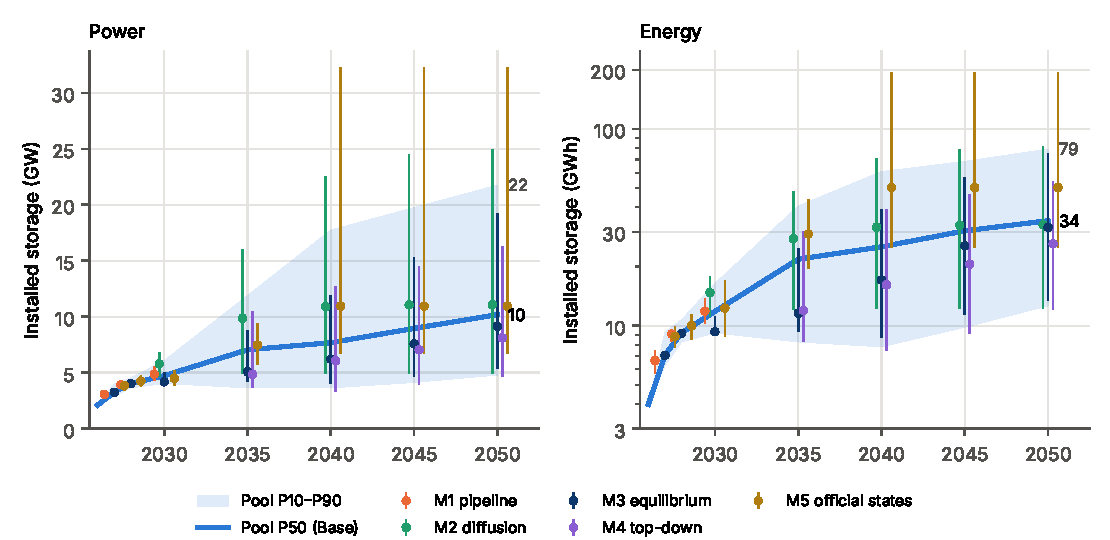
\includegraphics[width=\linewidth]{fig_forecast.pdf}
\caption{Pooled planning states (band: P10--P90; line: P50) with each method's median and P10--P90 at the pooled checkpoints. Energy is shown on a logarithmic axis.}
\label{fig:forecast}
\end{figure}

\subsection{What each method says}
Table~\ref{tab:methods} shows the methods separately.
To 2030 their medians lie within 2\,GW of each other: the queue method gives \val{m-M1-gw-p50-2030}\,GW, the published states \val{m-M5-gw-p50-2030} and the equilibrium \val{m-M3-gw-p50-2030}, because most of what will operate in 2030 is already committed.
By 2035 they have separated into two groups. Diffusion and the published states give \val{m-M2-gw-p50-2035} and \val{m-M5-gw-p50-2035}\,GW, while the equilibrium and the top-down method give \val{m-M3-gw-p50-2035} and \val{m-M4-gw-p50-2035}\,GW.
The economic method thus lies \emph{below} Fingrid's 2035 Moderate state of 6\,GW; its central path (\val{m3c-gw-2035}\,GW) reaches about 6\,GW only with cheap capital, demand led by data centres or weak cannibalisation, and not with fast technology learning alone (Section~\ref{sec:stress}).
The trend and institutional views therefore imply cheaper finance, faster growth of flexibility need or a fleet that erodes its own revenue less than the European evidence suggests.
This is the clearest disagreement in the forecast and the main reason the Low--High range for 2035 is wide.
By 2050 the economic and top-down methods give \val{m-M3-gw-p50-2050} and \val{m-M4-gw-p50-2050}\,GW, while the saturation prior and the vision states give about 11\,GW.

\begin{table}[t]
\centering
\caption{Method medians with P10--P90 at the pooled checkpoints: power in GW (upper block) and energy in GWh (lower block). A dash marks a checkpoint at which the method is not pooled.}
\label{tab:methods}
\small
\begin{tabular}{@{}lccccc@{}}
\toprule
Method & 2030 & 2035 & 2040 & 2045 & 2050\\
\midrule
\tabinput{generated/tab_methods.tex}
\bottomrule
\end{tabular}
\end{table}

\subsection{Duration: two hours today, four hours from the mid-2030s}
In the equilibrium the duration of new systems is an output.
Four-hour systems are the most profitable choice in \val{m3d4-2030}\,\% of draws in 2030, \val{m3d4-2035}\,\% in 2035, \val{m3d4-2040}\,\% in 2040 and \val{m3d4-2050}\,\% in 2050, and eight-hour systems in at most \val{m3d8-2050}\,\%. Along the central path, new builds switch from 2\,h to 4\,h in \val{m3c-first4h}.
Because the fleet of today and the committed tranche are short, the pooled fleet still averages only \val{st-dur-base-2035}\,h in 2035 and \val{st-dur-base-2050}\,h in 2050.

Two forces decide the switch. On the value side, the measured day-ahead margin rises from \val{dam-2} to \val{dam-4}\,k\EUR/MW between 2 and 4\,h, while the reserve and balancing pool pays per MW rather than per MWh and therefore favours short systems. On the cost side, the extra hour becomes cheaper as batteries learn and grid connection does not (Section~\ref{sec:cost}), and in 2026 the two extra hours still add more to annualised cost ($+$\val{ann-inc-24-2026}\,k\EUR/MW per year, from \val{ann-2-2026} to \val{ann-4-2026}) than to the day-ahead margin ($+$\val{dam-inc-24}\,k\EUR/MW per year with perfect foresight, or $+$\val{dam-inc-24-cap} at the central capture of \val{capture-central}).
When reserve revenue disappears or multi-hour spreads widen, 4\,h systems win earlier; when cannibalisation is applied to fleet energy rather than power, short systems remain the best choice (Table~\ref{tab:stress}).
Fingrid's lower bound of 4\,MWh/MW is therefore consistent with the economics for new systems from the mid-2030s, but not for the fleet as a whole by 2035, and 8\,h systems are not supported by today's Finnish price structure. The upper part of the 4--8\,h assumption in Fingrid's scenarios, and the Danish Energy Agency's 6\,h by 2050, are assumptions about how prices will be formed in the future, and they should be presented as such.
The difference matters for planning: at the 2035 Base power of \val{st-gw-base-2035}\,GW, the gap between a fleet of \val{st-dur-base-2035}\,h and one of 6\,h is about 20\,GWh.

\subsection{Stored energy and electricity use}\label{sec:use}
Today's \val{start-gwh}\,GWh corresponds to \val{min-load-now} minutes of average Finnish load. In the Base this rises to \val{use-minutes-p50-2030} minutes in 2030, \val{use-minutes-p50-2035} in 2035 and \val{use-minutes-p50-2050} in 2050 (Table~\ref{tab:use} and Figure~\ref{fig:use}).
Batteries therefore remain an intraday resource. Even the High state stores only about four hours of average load, far short of the multi-day cold and windless periods that Fingrid expects firm capacity to cover \citep{fingrid2026prospects}.

The fleet's own electricity use, consisting of conversion losses and auxiliary consumption, is \val{use-net-p50-2030}\,TWh in 2030, \val{use-net-p50-2035}\,TWh in 2035 and \val{use-net-p50-2050}\,TWh in 2050 at the median, or about \val{use-share-p50-2035}--\val{use-share-p50-2050}\,\% of national consumption.
Auxiliaries make up \val{aux-share-2050}\,\% of the 2050 total. Because they do not fall with throughput, the efficiency of heating, cooling and standby matters nearly as much as round-trip efficiency, and a lightly used fleet in a saturated market loses relatively more.
Gross annual throughput rises from \val{use-throughput-p50-2030} to \val{use-throughput-p50-2050}\,TWh; it is reported separately and not compared with consumption (Section~\ref{sec:boundary}).

\begin{table}[t]
\centering
\caption{Fleet operation and electricity use (medians, with P10--P90 in parentheses). Throughput is discharged energy; net use is conversion losses plus auxiliaries; the share is net use relative to national consumption.}
\label{tab:use}
\small
\begin{tabular}{@{}lrrrlrl@{}}
\toprule
Year & Throughput & Losses & Aux. & Net use & Share & Stored energy\\
 & (TWh) & (TWh) & (TWh) & (TWh) & (\%) & (min of avg. load)\\
\midrule
\tabinput{generated/tab_use.tex}
\bottomrule
\end{tabular}
\end{table}

\begin{figure}[t]
\centering
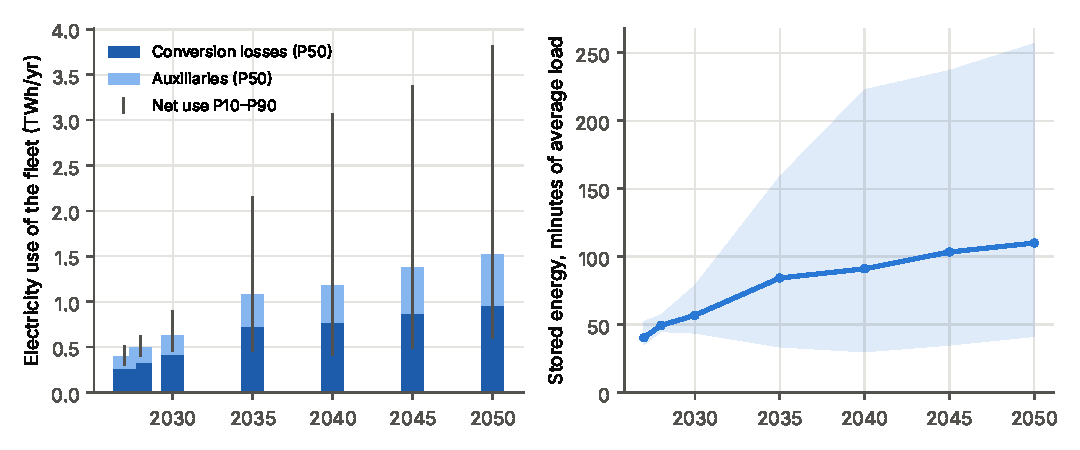
\includegraphics[width=\linewidth]{fig_electricity_use.pdf}
\caption{Fleet electricity use by component (left) and stored energy in minutes of average load (right), pooled states.}
\label{fig:use}
\end{figure}

\subsection{Cost per kWh and per MWh delivered}
The central installed cost of a 4\,h system, including grid connection, falls from \val{capex-4-2026}\,\EUR/kWh in 2026 to \val{capex-4-2035} in 2035 and \val{capex-4-2050} in 2050 (Table~\ref{tab:cost}).
Its levelised cost of storage at 250 cycles a year, excluding charging energy, falls from \val{lcos-4-2030}\,\EUR/MWh in 2030 to \val{lcos-4-2050} in 2050, and charging at the central price adds about \val{charge-adder}\,\EUR/MWh.
For a 4\,h system cycling once a day on arbitrage alone, the spread required to recover its annualised cost, measured as discharge price minus charging price divided by round-trip efficiency, falls from \val{be-4-2026}\,\EUR/MWh in 2026 to \val{be-4-2035} in 2035 and \val{be-4-2050} in 2050. The corresponding observed spread, the mean daily difference between the four most expensive hours and the four cheapest hours divided by efficiency, was \val{tbnet4-min}--\val{tbnet4-max}\,\EUR/MWh in 2023--2026 (\val{tb4-min}--\val{tb4-max} before efficiency losses). A 4\,h system that captured this spread every day would thus approach cost recovery on arbitrage alone in the mid-2030s, before allowing for imperfect foresight and for the fleet's own effect on spreads.

\section{Uncertainty and robustness}\label{sec:robust}

\subsection{Variance decomposition of the equilibrium}\label{sec:sobol}
First-order and total-effect Sobol indices of M3 are estimated with the estimators of \citet{saltelli2010variance} and \citet{jansen1999anova} from a base sample of \val{sobolbase}, or \val{sobol-evals} model evaluations (Table~\ref{tab:sobol} and Figure~\ref{fig:sobol}). Bootstrap standard errors are at most \val{sobol-se-max}; first-order estimates that exceed the total effect, or fall below zero, do so within that error.
The cost of the battery fleet enters through four separate dimensions, so that technology learning is not confounded with the cost of capital or with Finnish grid-connection costs.

Own-fleet cannibalisation dominates, with total effects of \val{sob-eps_own-2035-gw-ST} for power in 2035 and \val{sob-eps_own-2050-gw-ST} in 2050, followed by growth in flexibility need (\val{sob-eps_flex-2035-gw-ST} and \val{sob-eps_flex-2050-gw-ST}).
Among the cost dimensions, financing matters most (\val{sob-finance_u-2035-gw-ST} in 2035 and \val{sob-finance_u-2050-gw-ST} in 2050), followed by domestic project costs (\val{sob-project_u-2035-gw-ST} and \val{sob-project_u-2050-gw-ST}). The European premium (\val{sob-premium_u-2035-gw-ST} and \val{sob-premium_u-2050-gw-ST}) and the learning of globally traded components (\val{sob-cost_u-2035-gw-ST} and \val{sob-cost_u-2050-gw-ST}) contribute little.
Consumption level, the VRE multiplier, the size and shrinkage of the flexibility pool, pumped hydro, grid-forming units and the build-rate limit each stay below about 0.07.

The practical reading differs from the usual emphasis on battery prices. Once technology learning is separated from the cost of capital and from local project costs, the Finnish fleet is mostly a question of how the market prices the fleet's own presence and how fast the need for flexibility grows. Among costs, the cost of capital and the cost of connecting to the grid weigh more than the price of battery equipment, which is already a minority of the annualised cost and falls in every case. Finland shares fully in global technology learning, but that learning does not decide the size of its fleet.

\begin{table}[t]
\centering
\caption{Sobol indices of the equilibrium method (first order $S_1$, total effect $S_T$), ordered by the largest total effect. Bootstrap standard errors are at most \val{sobol-se-max}.}
\label{tab:sobol}
\small
\begin{tabular}{@{}lcccccccc@{}}
\toprule
 & \multicolumn{2}{c}{GW 2035} & \multicolumn{2}{c}{GWh 2035} & \multicolumn{2}{c}{GW 2050} & \multicolumn{2}{c}{GWh 2050}\\
\cmidrule(lr){2-3}\cmidrule(lr){4-5}\cmidrule(lr){6-7}\cmidrule(lr){8-9}
Parameter & $S_1$ & $S_T$ & $S_1$ & $S_T$ & $S_1$ & $S_T$ & $S_1$ & $S_T$\\
\midrule
\tabinput{generated/tab_sobol.tex}
\bottomrule
\end{tabular}
\end{table}

\begin{figure}[t]
\centering
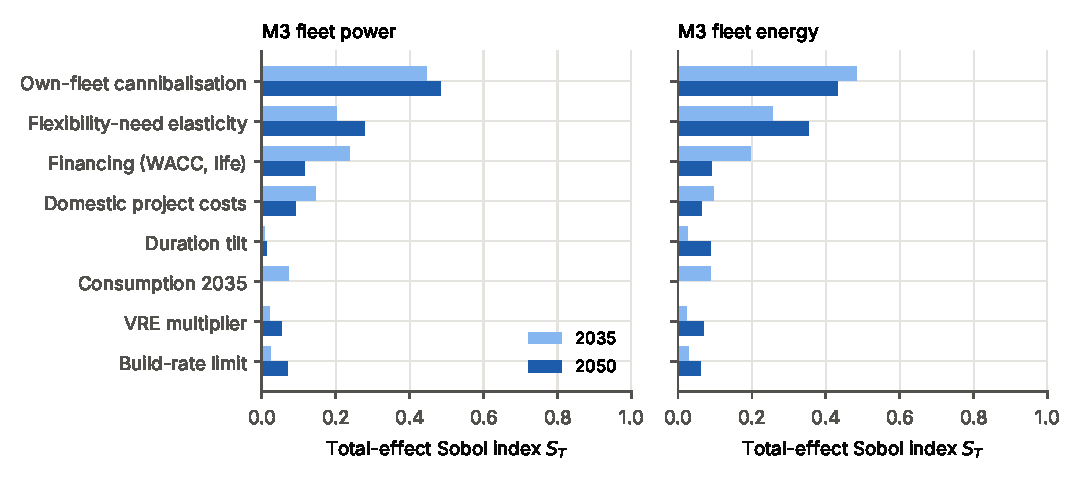
\includegraphics[width=\linewidth]{fig_sobol.pdf}
\caption{Total-effect Sobol indices of the equilibrium method for fleet power (left) and energy (right), 2035 and 2050.}
\label{fig:sobol}
\end{figure}

\subsection{Stress cases}\label{sec:stress}
Table~\ref{tab:stress} changes one input of the equilibrium at a time from its central configuration, whose path is \val{stress-central-gw-2035}\,GW in 2035 and \val{stress-central-gw-2050}\,GW in 2050.
Several pessimistic cases end at about \val{stress-dearcapital-gw-2035}\,GW in 2035, which is the committed stock: the market adds nothing beyond the projects already decided.
Technology alone moves the fleet little. Slow and fast global learning give \val{stress-slowgloballearning-gw-2050} and \val{stress-fastgloballearning-gw-2050}\,GW in 2050, a post-lithium chemistry that halves cell cost from 2030 gives \val{stress-postlithiumchemistrycells50from2030andbetterperformance-gw-2050}\,GW, and even free cells give only \val{stress-boundcellsfreeofchargefrom2030-gw-2050}\,GW. Fast convergence of the European premium gives \val{stress-fastpremiumconvergence-gw-2050}\,GW.
Finance and local costs move it more. Cheap capital (5\,\% and a 25-year life) gives \val{stress-cheapcapital-gw-2035}\,GW in 2035 and \val{stress-cheapcapital-gw-2050}\,GW in 2050, and grid connection at 100\,\EUR/kW gives \val{stress-lowdomesticprojectcosts-gw-2050}\,GW; dear capital or connection at 250\,\EUR/kW leave the fleet at \val{stress-dearcapital-gw-2050} and \val{stress-highdomesticprojectcosts-gw-2050}\,GW in 2050.
The market elasticities move it most. Weak cannibalisation gives \val{stress-weakcannibalisation-gw-2035}\,GW in 2035 and \val{stress-weakcannibalisation-gw-2050}\,GW in 2050, and demand led by data centres, with consumption reaching 200\,TWh and a 60\,\% higher VRE share, gives \val{stress-datacentreleddemand-gw-2035} and \val{stress-datacentreleddemand-gw-2050}\,GW.
Applying cannibalisation to fleet energy rather than power gives a similar fleet (\val{stress-arbitragecannibalisedbyenergy-gw-2050}\,GW in 2050) but keeps new builds short, because a longer battery then erodes its own spread faster.
Without shrinkage of the flexibility pool the 2050 fleet is \val{stress-noshrinkageoftheflexibilitypool-gw-2050}\,GW, with strong shrinkage \val{stress-strongshrinkageoftheflexibilitypool-gw-2050}\,GW. Moving from no pumped hydro to both Lapland projects reduces 2050 battery power from \val{stress-nopumpedhydro-gw-2050} to \val{stress-bothpumpedhydroprojects-gw-2050}\,GW.
None of the stress cases reaches Fingrid's 31\,GW vision state. That state rests on a demand-side driver, data-centre load combined with fully flexible electric boilers, that lies outside the revenue model of the equilibrium \citep{fingrid2025vision2040}.

\begin{table}[t]
\centering
\caption{Stress cases: one input of the equilibrium changed at a time from the central path. The post-lithium case also raises efficiency and cycle life and cuts auxiliary load; cycle life has no effect because calendar life binds at Finnish utilisation.}
\label{tab:stress}
\footnotesize
\begin{tabular}{@{}>{\raggedright\arraybackslash}p{6.6cm}rrrrcc@{}}
\toprule
 & \multicolumn{2}{c}{2035} & \multicolumn{2}{c}{2050} & New-build & First year\\
\cmidrule(lr){2-3}\cmidrule(lr){4-5}
Case & GW & GWh & GW & GWh & h, 2050 & of 4\,h\\
\midrule
\tabinput{generated/tab_stress.tex}
\bottomrule
\end{tabular}
\end{table}

\subsection{Pooling rule and seed stability}
Table~\ref{tab:loo} removes one method at a time. From 2035 onwards the Base median moves by at most \val{loo-max-late}\,\%; the largest shift arises when the economic method is removed in 2040, the checkpoint at which the remaining methods diverge most. Removing the economic method raises the Base, and removing the published states or the diffusion method lowers it.
Quantile averaging gives \val{vin-p50-2035}\,GW in 2035 and \val{vin-p50-2050}\,GW in 2050, against pool medians of \val{st-gw-base-2035} and \val{st-gw-base-2050}\,GW.
Table~\ref{tab:poolsens} shows the pooled states under the alternatives discussed in Section~\ref{sec:methods}. Scaling the Nordic peers by electricity consumption rather than population raises the 2050 Base to \val{poolsens1-base-2050}\,GW, and dropping the half weights of the diffusion and published-state methods raises the 2050 High from \val{poolsens0-high-2050} to \val{poolsens3-high-2050}\,GW.
Neither check changes the ordering of the states or their interpretation.
Across five independent seeds the Base varies by at most \val{seed-base-max}\,\% and the High by at most \val{seed-high-max}\,\%.

\begin{table}[t]
\centering
\caption{Shift of the pooled median power when one method is left out (\%), and the quantile-averaged (Vincentised) median.}
\label{tab:loo}
\small
\begin{tabular}{@{}lrrrrrrr@{}}
\toprule
Year & Base (GW) & $-$M1 & $-$M2 & $-$M3 & $-$M4 & $-$M5 & Vincent P50 (GW)\\
\midrule
\tabinput{generated/tab_loo.tex}
\bottomrule
\end{tabular}
\end{table}

\begin{table}[t]
\centering
\caption{Pooled states (GW) under alternative pooling and peer normalisation, and the median of the top-down method in 2050.}
\label{tab:poolsens}
\small
\begin{tabular}{@{}>{\raggedright\arraybackslash}p{5.6cm}rrrrrrr@{}}
\toprule
 & \multicolumn{3}{c}{2035} & \multicolumn{3}{c}{2050} & M4\\
\cmidrule(lr){2-4}\cmidrule(lr){5-7}
Variant & Low & Base & High & Low & Base & High & P50 2050\\
\midrule
\tabinput{generated/tab_poolsens.tex}
\bottomrule
\end{tabular}
\end{table}

\subsection{Sensitivity to the model specification}\label{sec:revision}
A simpler specification of the same framework uses a single equipment index with one bundled cost uncertainty and a high case without learning, a 15-year life and 6\,000 cycles without augmentation, higher auxiliary consumption, charges cell wear against day-ahead margins in addition to capital recovery, keeps the reserve pool fixed, retires units by continuous Weibull survival from installation, and pools all methods with equal weight.
Table~\ref{tab:revision} compares its results with the present model.
Installed cost is higher in the present model, mainly because augmentation is included, but annualised cost is lower because of the longer economic and cycle life. Day-ahead margins are higher once wear is not counted twice, which raises the equilibrium and moves new builds to 4\,h about a decade earlier.
The pooled Base barely moves. The Low state is higher, because warranted lives remove early retirements, and the High state is lower, because the two methods that share Fingrid's 2040 anchor do not count twice. The planning states are therefore robust to these specification choices, whereas the duration of new builds is not.

\begin{table}[t]
\centering
\caption{Results of the simpler specification and of the present model.}
\label{tab:revision}
\small
\begin{tabular}{@{}lrrr@{}}
\toprule
Quantity & Simpler specification & Present model & Change\\
\midrule
\tabinput{generated/tab_revision.tex}
\bottomrule
\end{tabular}
\end{table}

% =====================================================================
\section{Discussion}\label{sec:discussion}

Fingrid's 6--9\,GW for 2035 sits between the economics and the trend.
The Base is consistent with it because the pool includes trend and institutional views that the economics does not fully support.
If the fleet erodes its own margins at the elasticity found across Europe and capital costs about 7\,\%, the equilibrium points to about 5\,GW in 2035.
Reaching 6--9\,GW then requires weaker cannibalisation than the European evidence suggests, cheaper capital or cheaper grid connections, faster growth in flexibility need, or revenue that this model does not capture (intraday trading, capacity remuneration or co-location value). Faster technology learning alone is not enough.

Four observable quantities would move the states, and they can serve as leading indicators.
The first is the annual reserve and balancing pool, against \val{totpool-2026}\,M\EUR{} in 2026, together with day-ahead spreads as the fleet grows, which together show how strongly the fleet erodes its own revenue.
The second is the cost of capital for storage projects and the charges for connecting to the grid, which weigh more than equipment prices.
The third is the duration of new investment decisions, which the economics expects to shift to 4\,h in the mid-2030s.
The fourth is the commissioning of the 2027--2028 tranche. The 2027 Base of \val{st-gw-base-2027}\,GW lies below the market review's 3.6\,GW because it allows for slippage, so the review's 2027 figure is best read as an on-schedule state rather than a median.

For adequacy and for system planning, energy and duration matter more than power.
On the evidence here, the Finnish fleet will hold tens of GWh, not the hundreds that a 31\,GW fleet of 8\,h batteries would imply, unless price shapes change structurally.

% =====================================================================
\section{What this model does not do}\label{sec:limits}

The equilibrium scales measured margins with elasticities; it does not compute hourly prices from wind, solar, nuclear, interconnectors, data-centre load and competing flexibility.
Three simplifications follow from this. Cannibalisation acts on fleet power, whereas day-ahead spreads flatten with shifted energy; the stress case that applies it to energy gives a similar fleet but shorter batteries. Flexibility need grows with total consumption, although much of the new load (electric boilers, electrolysers) is itself flexible and may compress spreads; the low end of $\varepsilon_{\mathrm{flex}}$ covers this only approximately. The pool's response to the fleet is a single elasticity, whereas reserve prices may collapse non-linearly once a product is saturated.
A future version should replace Equation~\eqref{eq:rev} with a dispatch model over representative weather years, including the multi-day cold and windless periods to which batteries contribute only a bounded amount \citep{ieso2025elcc}.

The revenue streams are incomplete. The model uses perfect-foresight day-ahead margins scaled by a capture factor, together with the reserve and balancing pools. It does not represent continuous intraday trading, capacity remuneration such as the technology-neutral support under preparation \citep{tem2025flex}, congestion revenue, the value of co-location with wind and solar, or product redesign such as the Nordic limits on static FCR-D resources.

The long-horizon methods carry priors. After about 2038 the diffusion method returns its saturation prior, and the published-state method holds Fingrid's 2040 states flat; because both rest on Fingrid's 2040 vision, they share one method's weight from 2040. The top-down method is a mixture of two disjoint sub-methods in 2050, and its pooled contribution depends on how the Nordic peers are normalised (Table~\ref{tab:poolsens}).
Percentiles of the pool are not scenario paths: the Low state dips when the top-down method enters at the committed floor in 2035 and when the first-generation units pass their warranted life around 2040.

Some inputs are secondary or missing. The IEA's battery figures for 2030--2035, the Swedish peer value and the Italian auxiliary measurements were available only through secondary reporting at the cutoff. BloombergNEF's December 2026 price survey, which will show whether the European premium kept narrowing through the 2026 price rebound, was not yet published. Currency conversions use annual average rates assumed for 2024--2026. Demand for lithium-ion batteries after 2035, which sets the number of doublings, has no sourced outlook and is an assumption.

Distributed and mobile storage lies outside the estimand. The road-transport study's 2050 fleet implies onboard storage of the order of 100\,GWh \citep{merilehto2026road}, more than the stationary Base; how much of it would be available to the grid is a separate question.

% =====================================================================
\section{Conclusion}\label{sec:conclusion}
Finland's battery fleet grew past every official expectation in 2026 while its reserve-market revenue shrank.
Pooling five methods over the horizons on which each is informative gives a Base of \val{st-gw-base-2030}\,GW and \val{st-gwh-base-2030}\,GWh in 2030 (Low--High \val{st-gw-low-2030}--\val{st-gw-high-2030}\,GW), \val{st-gw-base-2035}\,GW and \val{st-gwh-base-2035}\,GWh in 2035 (\val{st-gw-low-2035}--\val{st-gw-high-2035}\,GW), and \val{st-gw-base-2050}\,GW and \val{st-gwh-base-2050}\,GWh in 2050 (\val{st-gw-low-2050}--\val{st-gw-high-2050}\,GW).

Three observations may carry beyond the numbers.
The first is that the near term is committed while the long term is a question of market design and finance more than of technology. The 2028 state is set by decisions already taken. The 2035 and 2050 states depend mostly on how the market prices the fleet's own presence and how fast the need for flexibility grows, and among costs on the cost of capital and of grid connection. Finland shares fully in global battery learning, but equipment is a shrinking share of the cost, and even free cells would add little.
The second is that duration is the hidden assumption of system planning. Under measured Finnish price shapes, two-hour systems are the economic choice today and four-hour systems from the mid-2030s, but eight-hour systems rarely pay, and the fleet as a whole stays near three hours. A fleet of 4--8\,h batteries is an assumption about future price formation rather than a consequence of today's market.
The third is that batteries remain an intraday resource with a small energy footprint. Even in 2050 the Base stores about two hours of average load, and its losses and auxiliary consumption draw about one per cent of national electricity.

Each of these conditions will become observable well before 2050, in the size of the flexibility pool and the spreads the fleet leaves itself, in the cost of capital and grid connection, in the durations of new investment decisions and in the commissioning of the committed tranche, and the framework released with this paper can be updated as each of them is observed.

\section*{Data and code availability}
The model source, executable parameter set, derived data, figure code and test suite are released at \url{https://github.com/juhanimerilehto/bess-finland-2050} (MIT licence for code, CC~BY~4.0 for text, figures and data) and archived with this paper at \href{https://doi.org/10.5281/zenodo.24322467}{doi:10.5281/zenodo.24322467}.
Every model-derived number in the text, tables and figures is written by the model run, so the text cannot drift from the outputs \citep{pfenninger2017open}.
The Zenodo archive also holds the snapshot of Fingrid open data (CC~BY~4.0) used here. Day-ahead prices are retrieved from the ENTSO-E Transparency Platform by the included script with the user's own security token, and a manifest of SHA-256 checksums shows whether a fresh download matches the snapshot used in the paper.
Without the raw data, the run rebuilds the forecast, tables and figures from the derived market series in the release; with them, every step runs from the raw series:
\begin{verbatim}
python model/fetch_fingrid.py          # not needed with the Zenodo archive
python model/fetch_entsoe.py --only da
python model/run_all.py
python -m unittest discover -s model/tests
latexmk -cd -pdf paper/bess_finland_2050.tex
\end{verbatim}
Only Python with NumPy, SciPy and Matplotlib is required, and the run is deterministic given the recorded seed.
The SHA-256 prefixes of the files are \texttt{\val{params-sha}} for the parameter file, \texttt{\val{sha-fequilibrium}} for the equilibrium module, \texttt{\val{sha-fmethods}} for the method module, \texttt{\val{sha-ensemble}} for the pooling module and \texttt{\val{sha-cost}} for the cost module.
The test suite checks exact reproduction of the market review's and Fingrid's states, the cost anchor against BloombergNEF, the component model's reproduction of BloombergNEF's 2035 European price, its agreement with the published-forecast path, the ordering of the European-premium cases, the cycle-cost range, the separation of the four cost dimensions and the two contract validations, M1's 2028 median and M2's anchors, M5's published medians, the committed floor, a Base inside Fingrid's 2030 and 2035 ranges, monotone Base states, and the calibration of the equilibrium to the 2026 fleet.

\bibliographystyle{plainnat}
\bibliography{refs}

\clearpage
\appendix
\section{Parameter set}\label{app:params}

{\footnotesize
\begin{xltabular}{\linewidth}{@{}>{\raggedright\arraybackslash}p{4.3cm}>{\raggedright\arraybackslash}p{3.2cm}l>{\raggedright\arraybackslash}X@{}}
\caption{Model parameters: low / central / high (triangular unless stated; cost parameters listed from low-cost to high-cost case) and evidence class.}
\label{tab:params}\\
\toprule
Parameter & Low / central / high & Class & Anchor\\
\midrule
\endfirsthead
\toprule
Parameter & Low / central / high & Class & Anchor\\
\midrule
\endhead
\multicolumn{4}{@{}l}{\emph{Start and project queue (M1)}}\\
Stock, Nov 2026 & 2.092\,GW; 3.97\,GWh & \cls{m}/\cls{a} & Fingrid 424; 1.9\,h assumed\\
FID tranche & 1.808\,GW, 2.8\,h; $p$ 0.85/0.95/1 & \cls{v}/\cls{a} & Market review: 3.9\,GW operating + FID by end-2028\\
Permitted, net & 0.887\,GW; $p$ 0.3/0.5/0.7 & \cls{s}/\cls{a} & Renewables Finland: 1.7\,GW permitted\\
Early planning & 9.2\,GW, 3.0\,h; $p$ 0.05/0.15/0.30 & \cls{s}/\cls{a} & 11.9\,GW / 36\,GWh planned\\
\multicolumn{4}{@{}l}{\emph{Diffusion (M2)}}\\
Saturation $K$ & 4--31\,GW, log-uniform & \cls{f}/\cls{a} & Fingrid 2030 Moderate; vision maximum\\
\multicolumn{4}{@{}l}{\emph{Equilibrium (M3)}}\\
Capture $\kappa$ & 0.75 / 0.85 / 0.95 & \cls{a} & Perfect-foresight overstatement\\
$\varepsilon_{\mathrm{own}}$ & 0.3 / 0.8 / 1.2 & \cls{b}/\cls{a} & \citet{savelli2026cannibalisation}; \citet{seville2026spain}\\
$\varepsilon_{\mathrm{flex}}$ & 0.3 / 0.8 / 1.5 & \cls{b}/\cls{a} & \citet{savelli2026cannibalisation}; \citet{dumitrescu2024price}\\
$\varepsilon_{\mathrm{pool}}$ & 0 / 0.5 / 1 & \cls{a} & Reserve need grows with VRE and loads\\
$\varepsilon_{\mathrm{sat}}$ (pool shrinkage) & 0.2 / 0.5 / 0.9 & \cls{m}/\cls{a} & Pool halved as fleet doubled, 2025--2026\\
Battery pool share $s$ & 0.3 / 0.5 / 0.8 & \cls{a} & Hydro, boilers, demand compete\\
Pool $P_0$ & 124.7\,M\EUR & \cls{m} & Table~\ref{tab:market}, 2026\\
Pool eligibility $e_d$ & 0.4 (1\,h); 1 otherwise & \cls{s}/\cls{a} & Endurance rules \citep{nordictsos2025batteries}\\
Consumption 2035 & 110 / 136 / 162\,TWh & \cls{f} & \citet{fingrid2026prospects}\\
Consumption 2050 & 134 / 155 / 200\,TWh & \cls{f}/\cls{a} & Climate plan; data-centre tail\\
VRE multiplier 2050 & 1.0 / 1.3 / 1.6 & \cls{a} & \\
Duration tilt $\tau$ & 0 / 0.15 / 0.3 & \cls{a} & Fingrid 4--8\,h; DEA 6\,h; \citet{landy2026hybrids}\\
Build limit & 0.6 / 1.2 / 2.5\,GW/yr & \cls{m}/\cls{a} & 2026: $+$1.2\,GW/yr observed\\
Connection cap & 31\,GW & \cls{f} & Vision maximum; $>$30\,GW enquiries\\
Pumped hydro & 0 / 0.55 / 1.05\,GW (p 0.3/0.4/0.3) & \cls{v}/\cls{a} & Kemijoki 2033; PVO 2036\\
Grid-forming units 2050 & 0 / 0.8 / 3.0\,GW & \cls{s}/\cls{a} & Grid-code weak-grid rule\\
Retirement & none before 10\,yr; Weibull, shape 3, mean life 15\,yr (2025) $\to$ 20\,yr (2050) & \cls{v}/\cls{f}/\cls{a} & Warranties; NREL 15\,yr; Lazard 20\,yr\\
Cannibalisation basis & fleet power (central); fleet energy (stress) & \cls{a} & \citet{savelli2026cannibalisation}\\
\multicolumn{4}{@{}l}{\emph{Cost and technology (component model): technology-learning dimension}}\\
Cells, EXW China 2025 & 36\,EUR/kWh & \cls{b} & Ember; BNEF lowest LFP cell\\
Cell learning rate & 21 / 18 / 15\,\% per doubling & \cls{m} & \citet{ziegler2021rates}\\
Global Li-ion doublings 2035 / 2050 & 3.7 / 3.3 / 3.0; 5.6 / 5.1 / 4.65 & \cls{a} & 4.7\,TWh cumulative end-2025; IEA-type outlooks\\
Cell materials floor & 12 / 18 / 28\,EUR/kWh & \cls{a} & cathode incl. lithium 42--46\,\% of cell cost\\
DC BOS and PCS learning rate & 15 / 12 / 8\,\% per doubling & \cls{b}/\cls{a} & NREL component path; \citet{schmidt2017experience}\\
Near-term index 2026 / 2027 (hardware) & 0.95--1.10 / 0.90--1.08 & \cls{m}/\cls{a} & 2026 rebound; export rebate removal\\
Augmentation allowance & 5--20\,\% (2025) to 2.5--10\,\% (2050) & \cls{b}/\cls{a} & industry practice\\
High-case lithium premium on cells & $+$20\,\% at 2030, zero in 2025 and 2035 & \cls{a} & 2021--22 and 2026 price spikes\\
\multicolumn{4}{@{}l}{\emph{European-premium dimension}}\\
European premium 2025 & 69.5\,EUR/kWh & \cls{b} & residual of BNEF Europe turnkey\\
Premium decline to / after 2035 & 10 / 5 / 2\,\% and 3 / 2 / 1\,\% per yr & \cls{f}/\cls{a} & BNEF 2035 Europe and China outlook\\
\multicolumn{4}{@{}l}{\emph{Domestic-project-cost dimension}}\\
Installation (share of 2025 equipment) & 15\,\%, $-$2 / $-$1 / 0\,\% per yr & \cls{a} & Ember installation and connection split\\
Grid connection & 100 / 150 / 250\,EUR/kW, flat & \cls{b}/\cls{a} & Ember; Danish Energy Agency\\
Fixed O\&M & 1 / 2 / 3\,\% of equipment and installation & \cls{b}/\cls{a} & NREL; Lazard\\
Auxiliaries (2025 $\to$ 2050) & 0.9 / 1.8 / 3.3\,kW/MWh, $-$28\,\% by 2050 & \cls{b}/\cls{a} & Section~\ref{sec:tech}\\
\multicolumn{4}{@{}l}{\emph{Performance (not sampled separately)}}\\
Cycle life (2025 vintage $\to$ 2050) & 12\,000 / 8\,000 / 6\,000 $\to$ 20\,000 / 15\,000 / 10\,000 & \cls{v}/\cls{b} & PNNL; vendor terms; field fade\\
Round-trip efficiency (AC, excl. aux.) & 0.89 / 0.85 / 0.82, $+$3\,pp by 2050 & \cls{b} & PNNL; NREL; Lazard\\
\multicolumn{4}{@{}l}{\emph{Financing dimension}}\\
Real WACC with economic life & 5\,\% and 25\,yr / 7\,\% and 20\,yr / 10\,\% and 15\,yr & \cls{a}/\cls{v} & vendor warranties; Lazard; NREL\\
\multicolumn{4}{@{}l}{\emph{Top-down (M4)}}\\
Global fleet 2030 / 2035 / 2050 & 900--1\,200 / 1\,400--2\,900 / 3\,800--4\,100\,GW & \cls{f} & Table~\ref{tab:external}\\
Finnish share 2050 & 0.25 / 0.35 / 0.50\,\% & \cls{a} & 0.46\,\% today\\
Peers 2050 & DK 1.14; SE 0.78--0.89\,kW/cap, scaled by population & \cls{f} & DEA AF25; Svk LMA2026 (secondary)\\
\multicolumn{4}{@{}l}{\emph{Pooling}}\\
Method weights & equal; M2 and M5 at 0.5 from 2040 & \cls{a} & Shared Fingrid 2040 anchor\\
\multicolumn{4}{@{}l}{\emph{Energy and operation}}\\
New-build $h$ 2050 (M1, M2, M4) & 2 / 4 / 8 & \cls{f}/\cls{a} & M3; Fingrid\\
Scenario additions (M5) & 4--8\,h uniform & \cls{f} & \citet{fingrid2026prospects}\\
Cycles per year & 150 / 220 / 330 & \cls{m}/\cls{a} & Fingrid 398, Jun--Oct 2026\\
\bottomrule
\end{xltabular}
}

\section{External forecast compilation}\label{app:external}

\begin{table}[H]
\centering
\caption{Selected external forecasts and states. Cumulative installed capacity unless stated. Access: P read in the publisher's document; S secondary reporting only.}
\label{tab:external}
\footnotesize
\begin{tabularx}{\linewidth}{@{}>{\raggedright\arraybackslash}X l l >{\raggedright\arraybackslash}p{5.2cm} c@{}}
\toprule
Source & Published & Scope & Values & Access\\
\midrule
BNEF NEO 2026, ETS \citep{bnef2026neo} & May 2026 & Global & 2\,011\,GW (2035); 3\,844\,GW (2050) & P\\
BNEF ESMO 2H 2026 \citep{bnef2026esmo} & Oct 2026 & Global & 3\,098\,GW / 11.1\,TWh (2036) & S\\
IEA WEO 2025 \citep{iea2025weo} & Nov 2025 & Global & $\sim$900\,GW (2030, STEPS); 1\,400 / 1\,700 / 2\,900\,GW (2035, CPS/STEPS/NZE) & S\\
IRENA WETO 2024, 1.5\,$^\circ$C \citep{irena2024weto} & Nov 2024 & Global & 4\,100\,GW (2050) & P\\
CNESA White Paper 2026 \citep{cnesa2026white} & May 2026 & China & 371--451\,GW new-type (2030); avg. duration 3.47\,h (2030) & P\\
Danish Energy Agency AF25 \citep{dea2025af25} & Nov 2025 & Denmark & $\sim$4.0\,GW (2030); $\sim$6.8\,GW (2050), 2\,h $\to$ 6\,h & P\\
Svenska kraftnät LMA2026 \citep{svk2026lma} & Jun 2026 & Sweden & 8.3--9.4\,GW (2050) & S\\
ENTSO-E ERAA 2023 & 2024 & Nordics & $\sim$1.8\,GW (2030) & S\\
Rabobank \citep{rabobank2026nordicbess} & Jul 2026 & Nordics & $\sim$5\,GW (2030) & P\\
Fingrid Q3/2026 \citep{fingrid2026prospects} & Sep 2026 & Finland & 4 / 5\,GW (2030); 6 / 9\,GW (2035), 4--8\,MWh/MW; High 2035 ``almost 50\,GWh'' & P\\
Fingrid vision 2040 \citep{fingrid2025vision2040} & Oct 2025 & Finland & 2 / 7 / 11 / 31\,GW (2040) & P\\
Fingrid vision 2023 \citep{fingrid2023vision} & 2023 & Finland & 1--4\,GW (2035); 1--6\,GW (2045) & P\\
Expert elicitation \citep{borenius2025bayesian} & 2025 & Finland & 1.1\,GW (2035), elicited 2024 & P\\
Merilehto (2026), market review \citep{merilehto2026blog} & Oct 2026 & Finland & 3.94\,GW (2027); 4.44\,GW (2028), project queue & P\\
Renewables Finland \citep{renewablesfi2026bess} & Sep 2026 & Finland & 0.995\,GW / 2.8\,GWh under construction; 11.9\,GW / 36\,GWh planned & P\\
\bottomrule
\end{tabularx}
\end{table}

\end{document}
